% Bachelor Thesis -- body only. The title page and statutory declaration are supplied
% separately; this file begins at the abstract and the table of contents.
%
% Result tables in thesis/tables/ are generated by scripts/make_thesis_tables.py directly from
% the experiment JSON, so no number in this document is transcribed by hand.
\documentclass[11pt,a4paper,oneside]{report}

\usepackage[utf8]{inputenc}
\usepackage[T1]{fontenc}
\usepackage{lmodern}
% Symmetric 2.5cm margins, the one-inch measure of the source paper. The asymmetric
% 3.5cm/2.5cm pair this replaced was a binding allowance, but it only alternates under the
% twoside option; in a oneside document it shifted every page right of centre. If the thesis
% is to be printed and bound, switch the class to twoside and use inner=3.5cm,outer=2.5cm.
\usepackage[top=2.5cm,bottom=2.5cm,left=2.5cm,right=2.5cm]{geometry}
\usepackage{amsmath,amssymb}
\usepackage{booktabs}
\usepackage{longtable}
\usepackage{graphicx}
\usepackage[font=footnotesize,labelfont=bf,skip=4pt]{caption}
\captionsetup{format=plain, justification=justified, singlelinecheck=false}

% Condensed float spacing. The class defaults reserve close to a line of body text above and
% below every float, which over nine figures and nine tables costs roughly a page.
\setlength{\textfloatsep}{6pt plus 2pt minus 3pt}
\setlength{\intextsep}{7pt plus 2pt minus 3pt}
\setlength{\floatsep}{7pt plus 2pt minus 3pt}
\setlength{\abovecaptionskip}{4pt}
\setlength{\belowcaptionskip}{2pt}
% The class reserves a fifth of every page for text before it will place a float there, and
% sends any float taller than half a page to a float-only page. Both defaults were costing
% whole pages here: Figure 4.6 alone occupied one. Raising the top/bottom fractions and the
% float-page threshold lets a tall float share a page with the text that discusses it.
\renewcommand{\topfraction}{0.92}
\renewcommand{\bottomfraction}{0.65}
\renewcommand{\textfraction}{0.08}
\renewcommand{\floatpagefraction}{0.82}
\setcounter{topnumber}{3}
\setcounter{bottomnumber}{2}
\setcounter{totalnumber}{4}
\usepackage{microtype}
\usepackage{setspace}
\onehalfspacing
\usepackage{tikz}
\usetikzlibrary{arrows.meta, positioning, fit, backgrounds, calc, shapes.geometric}
\usepackage{listings}
% The stock report chapter head reserves roughly a fifth of the first page of every chapter,
% and \onehalfspacing stretches a title that runs to two lines on top of that. The head is set
% single-spaced and the space above and below it reduced, which recovers the page without
% making the heading less prominent than the class intends.
\usepackage{titlesec}
\titleformat{\chapter}[display]
  {\normalfont\LARGE\bfseries\singlespacing}
  {\normalsize\bfseries\chaptertitlename\ \thechapter}{0.5em}{}
\titlespacing*{\chapter}{0pt}{-12pt}{24pt}
\titlespacing*{\section}{0pt}{1.6ex plus 0.4ex minus 0.2ex}{0.9ex plus 0.2ex}
\titlespacing*{\subsection}{0pt}{1.3ex plus 0.3ex minus 0.2ex}{0.7ex plus 0.2ex}

\usepackage[numbers,sort&compress]{natbib}
\usepackage[hidelinks,colorlinks=true,linkcolor=blue,citecolor=blue]{hyperref}

% ---- TikZ styles, shared by every diagram so the figures read as one family ----
% ---- Diagram styles -------------------------------------------------------------------
% Node text is set at \footnotesize and edge text at \scriptsize, both within one step of
% the 11pt body, so that no diagram depends on \resizebox to fit the text block. Boxes are
% given a common width where they sit in a row, so that rows align without manual shifts.
\tikzset{
  blk/.style   = {draw=black!70, rounded corners=2.5pt, align=center, inner sep=4.5pt,
                  font=\footnotesize, minimum height=10mm, line width=0.5pt},
  io/.style    = {blk, fill=black!4},
  core/.style  = {blk, fill=blue!10},
  head/.style  = {blk, fill=green!12},
  dp/.style    = {blk, fill=red!10},
  ev/.style    = {draw=black!70, circle, inner sep=1pt, minimum size=8mm,
                  font=\footnotesize, line width=0.5pt},
  fl/.style    = {-{Latex[length=2mm, width=1.6mm]}, line width=0.7pt, draw=black!70},
  crit/.style  = {line width=1.5pt, draw=black},
  slack/.style = {draw=black!40},
  elab/.style  = {font=\scriptsize, inner sep=1.5pt, fill=white, fill opacity=0.85,
                  text opacity=1},
  ntag/.style  = {font=\scriptsize, inner sep=1pt, text=black!65},
  panlab/.style= {font=\footnotesize\bfseries, inner sep=0pt},
  grp/.style   = {draw=black!35, dashed, rounded corners=4pt, inner sep=7pt},
}

% ---- Source listing style for the one code excerpt ----
% Styled to match the booktabs tables: horizontal rules only, no box, no vertical lines.
\lstdefinestyle{py}{
  basicstyle=\ttfamily\footnotesize\setstretch{1}, keywordstyle=\bfseries,
  commentstyle=\itshape\color{black!50}, stringstyle=\color{black!70},
  language=Python, showstringspaces=false,
  breaklines=false,                      % lines are kept short enough not to wrap
  frame=tb, framerule=0.8pt, rulecolor=\color{black}, framesep=6pt,
  aboveskip=1.2em, belowskip=1.2em,
  numbers=left, numberstyle=\tiny\color{black!40}, numbersep=9pt,
  xleftmargin=20pt, lineskip=1.2pt,
}

\setlength{\parskip}{0.18em}
\setlength{\parindent}{0pt}

% A handful of long hyphenated compounds and inline-math atoms cannot be broken, which produced
% three overfull boxes. emergencystretch lets TeX loosen those lines rather than run into the
% margin, and the hyphenation list supplies break points for the offending words.
\setlength{\emergencystretch}{1.5em}
\hyphenation{speed-adjust-able ex-plain-abil-ity at-ten-tion-weight-ed
             non-dom-i-nated multi-pop-u-la-tion het-ero-ge-neous
             sub-gra-di-ent trans-port-bound}

\newcommand{\Cmax}{C_{\max}}
\DeclareMathOperator*{\argmax}{arg\,max}

\begin{document}

% ======================================================================================
\chapter*{Abstract}
\addcontentsline{toc}{section}{Abstract}

Container terminals schedule quay cranes and speed-adjustable automated guided vehicles against
two conflicting objectives, the makespan of the workload and the energy consumed by the vehicles.
The solution is not a single schedule but a Pareto front of non-dominated compromises from which
an operator must select. The literature is substantially richer in methods that compute fronts
than in methods that explain them, and the explainability techniques usually transferred from
machine learning attribute outcomes to decision variables rather than to physical quantities on
which an operator can act.

This thesis explains Pareto-optimal schedules in terms of the physical activities that produce
them. The account rests on a structural observation: once a schedule is fixed, its makespan is
the longest chain of activities that must happen in sequence, so only the activities on that
chain can affect it, and their durations add up to the makespan exactly. The sensitivity of the
makespan to any activity is therefore one or zero rather than something in between, and the
resulting explanation balances by construction. Formally this is linearity over the $(\max,+)$
semiring, and it makes the explanation checkable rather than merely plausible. The method built on
it is a heterogeneous graph attention network, E-HGATv2, which encodes the schedule as a typed
precedence graph and predicts per-leg travel durations and per-task handling delays, which a
differentiable max-plus dynamic-programming layer composes into the makespan, its custom backward
pass routing the subgradient exclusively through the argmax edge of each recurrence.

From this decomposition the thesis defines the duration-weighted critical share $\rho$, the
fraction of the makespan contributed by vehicle travel rather than crane handling, and uses its
shift between the ends of a front to quantify why the compromises differ. The principal finding
is that the binding bottleneck migrates between travel and handling, and that whether it does is
governed by the fleet-to-crane ratio $A/Q$. Across 540 replicates spanning six instances, nine
fleet sizes and ten seeds, migration is significantly non-zero in 45 of 54 instance--fleet cells
under a Holm-corrected Wilcoxon signed-rank test, attaining $0.665$ at $A/Q = 2.67$ and vanishing
below $A/Q \approx 1$ where both ends are transport-bound. A second campaign of 8{,}640
replicates reproduces the threshold on three instance families and resolves the explanation at
all 657{,}899 points of the fronts it produces. Where the transfer occurs, cranes bind at the
makespan-optimal end and vehicles at the energy-optimal end, which accounts for its absence on
the ten published large instances, each having $A/Q = 0.50$. The surrogate reproduces the exact
explanation to a mean absolute error of $0.026$ in the share and a critical-leg agreement of
$0.898$ on the small instances and $0.924$ on the published large ones, and it does so at every
generation of a search as well as at its end. That agreement is what carries the method beyond
the cases examined here, since the exact recurrence can only be applied to a schedule that has
already been evaluated whereas the model predicts the durations it needs.

% ======================================================================================
\setcounter{tocdepth}{1}
{\singlespacing\setlength{\parskip}{0pt}\tableofcontents}
\cleardoublepage

% ======================================================================================
\chapter{Introduction}

A container terminal mediates between maritime and inland transport, and its throughput is
governed by the coordination of its equipment. Quay cranes transfer containers between vessel and
quay; automated guided vehicles transport them between quay and storage yard. Scheduling the two
resources jointly dominates scheduling them in sequence, because an idle crane represents
unrecovered capital and an idle vehicle represents wasted energy. Contemporary terminals
increasingly deploy vehicles whose travel speed is selectable, which introduces a second
objective: a vehicle driven faster completes its leg sooner but consumes disproportionately more
energy, since power grows super-linearly in speed.

The problem consequently admits no single optimum. It admits a Pareto front: a set of schedules,
none of which improves upon another in one objective without conceding the other.
\citet{fontes2023} formulate the problem as a bi-objective mixed-integer linear program and solve
it with a multi-population biased random-key genetic algorithm, reporting fronts for benchmark
instances of increasing size. Their contribution concerns the efficient computation of the front.

The subsequent question has received less attention. An operator receives a front and must
select from it. Selection presupposes understanding, and understanding a schedule requires knowing what
limits it. Two schedules on the same front may be limited by entirely different resources: one
may be constrained by vehicles traversing a long yard-to-quay distance, another by a single
overloaded crane whose task queue no increase in fleet size will shorten. These situations
require distinct operational responses, and the front alone does not distinguish them. The front
reports the magnitude of the trade-off; it does not report its cause.

\section{Significance}

Two questions are worth separating: whether a front can be computed, and whether it can be
understood. The first is settled for this problem; the second is what this thesis addresses, and
it matters for a practical reason. A front is not a recommendation. It is a menu, and the
operator who must choose from it is choosing between schedules that may fail for entirely
different reasons. If one compromise is slow because too few vehicles are covering a long yard,
buying a vehicle helps; if another is slow because a single crane has too many containers queued
against it, buying a vehicle changes nothing and the tasks must be rebalanced. The two look alike
on the front, because the front records only the makespan and the energy, never the reason. An
operator told which resource is binding at the point they are considering can act; an operator
given the two numbers alone can only guess.

The gap is not specific to container terminals. \citet{bengio2021} survey the integration of
machine learning with combinatorial optimisation and identify the interpretation of optimiser
output as a persistent weakness. Within multi-objective optimisation the usual devices are
indirect: fronts are visualised, which conveys the shape of a trade-off but not its cause;
solutions are clustered, which groups compromises without saying what distinguishes them; or a
preference is elicited and one solution recommended, which replaces one unanswered question with
another. Recent work applies post-hoc attribution, principally SHAP \citep{lundberg2017} and
TreeSHAP \citep{lundberg2020}, to surrogate models of the objective. In a scheduling context that
carries a specific limitation: the attribution lands on \emph{decision variables}, on positions
in a chromosome and on discrete speed settings, not on \emph{physical quantities}. Being told
that the twenty-seventh gene of a chromosome matters does not tell an operator what to do. Being
told that the loaded trip from crane three to yard station one lies on the critical path and
contributes $55.6$ seconds does.

\section{Novelty}

What makes the problem tractable here is a structural property rather than a new technique.
\citet{rudin2019} argues that where a model's structure permits an explanation that is correct by
construction, explaining an opaque model after the fact is the inferior choice. This problem
permits exactly that. The makespan of a fixed schedule is the largest total along any chain of
activities that must happen in order, which is to say it is the length of a longest path through
the schedule. Two consequences follow. Only the activities on that path can affect the makespan
at all, so the sensitivity of the makespan to any activity is either one or zero, never something
in between. And the durations of the activities on that path add up to the makespan exactly. The
explanation is therefore not fitted or approximated; it is read off the structure, and it
balances by construction. Formally this is linearity over the $(\max,+)$ semiring
\citep{baccelli1992}, developed in Section~\ref{sec:maxplus}.

The two ingredients this thesis combines are each established. Graph neural networks have been
applied to scheduling and routing, as policies \citep{kool2019, zhang2020} and as surrogates, and
differentiable optimisation layers embed a combinatorial computation inside a network so that
gradients pass through it \citep{amos2017, pogancic2020}, with the decision-focused learning
literature studying prediction whose loss is defined through a downstream optimiser
\citep{elmachtoub2022}. Their combination for this problem class is, to the author's knowledge,
not established. The novelty is in what the network is asked to predict. It does not predict the
makespan. It predicts the \emph{local physical quantities} of a schedule, the duration of each
vehicle trip and each crane lift, and a max-plus layer then composes those into the makespan
using the same recurrence the exact evaluator uses. Differentiating the model with respect to its
own predictions therefore returns the critical path itself rather than an estimate of it, and the
answer is expressed in seconds attributable to named activities rather than in units of an
internal representation.

\section{Contribution}

This thesis has one core idea: \emph{a Pareto-optimal schedule can be explained exactly, in
seconds attributable to named physical activities, and a learned model can produce that same
explanation}. Everything reported here serves that idea.

The explanation itself is exact rather than estimated. For a given schedule the method identifies
which vehicle trips and crane lifts actually determine the makespan, and how many seconds each
contributes. Because those durations add up to the makespan exactly, the explanation can be
checked rather than merely believed, and it is checked on every schedule reported, so an
inconsistency appears as a failed test rather than as a plausible figure. This holds because a
fixed schedule's makespan is the longest chain of activities that must run in sequence, which
makes the sensitivity to any one activity either one or zero.

The learned surrogate, E-HGATv2, is the supporting tool. It is not asked to predict the
makespan; it predicts the duration of each trip and each lift, and a differentiable max-plus
layer composes those into the makespan using the same recurrence the exact evaluator uses.
Differentiating the model with respect to its own predictions therefore returns a critical path
rather than an estimate of one, expressed in the same physical units. Whether it agrees with the
exact answer is measured throughout and reported in Section~\ref{sec:surrogate-eval}.

That the explanation is worth having at all is established by a single empirical fact: the answer
is not the same everywhere on a front. With enough vehicles the makespan-optimal end of a front
is limited by the cranes and the energy-optimal end by the vehicles, so two schedules an operator
is choosing between fail for different reasons and call for different interventions. Whether this
occurs is governed by the number of vehicles per crane, which is established by a statistically
tested sweep (Section~\ref{sec:migration}) and reproduced on three instance families. This is
evidence for the core idea rather than a second contribution: without it, explaining a schedule
would be a demonstration on one solution instead of a statement about the front.

Chapter~\ref{sec:motivation} states the problem, its formulation, the solution method and the
relevant background. Chapter~\ref{sec:method} describes the surrogate architecture, the max-plus
layer, the derived measure and the experimental design. Chapter~\ref{sec:evaluation} evaluates
the results, beginning with verification. Chapter~\ref{sec:limitations} states the limitations,
including one degenerate case the implementation does not handle correctly.
Chapter~\ref{sec:conclusion} concludes.

% ======================================================================================
\chapter{Problem Formulation and Background}
\label{sec:motivation}

\section{The problem, its entities and the physics of a leg}
\label{sec:entities}

An instance is a set of container moves (\emph{tasks}) $\mathcal{J} = \{0,\dots,N-1\}$, each bound
to one quay crane $\mathrm{qc}(j)$ with handling time $\tau_j$ and one yard station
$\mathrm{lu}(j)$, served by a fleet of $|\mathcal{A}|$ speed-adjustable vehicles. A task is of one
of two kinds. A \emph{loading} task ($j \in \mathcal{L}$, a LOAD) moves a container from yard to
vessel: a vehicle travels empty to the yard station, collects the container, carries it to the
crane, and the crane lifts it aboard, so its loaded leg runs $\mathrm{LU} \to \mathrm{QC}$. An
\emph{unloading} task ($j \in \mathcal{U}$, an UNLOAD) reverses this, the crane lifting a
container from the vessel onto a waiting vehicle which transports it to the yard. Each crane
processes its tasks one at a time.

A decision specifies, for every task, the assigned vehicle, its position in that vehicle's
sequence and in its crane's sequence, and a discrete \emph{speed level} for the empty leg and for
the loaded leg, one of a small fixed set of velocities at which a vehicle may be driven; a higher
level shortens the leg and raises its power draw. The instances follow the three-level
configuration of \citet{fontes2023}. Two objectives are minimised: the makespan $\Cmax$, the
completion time of all work, and the energy $E$ consumed by vehicle travel. Crane handling energy
is excluded from $E$, which is material to the interpretation of both objectives, since the crane
contributes to one and not the other.

Table~\ref{tab:notation} collects the notation. Sequencing is represented by the order of tasks
within a resource's chain, and the formulation below states the problem as the timing recurrences
a resolved schedule satisfies.

\begin{table}[tb]
\centering
\footnotesize
\caption[Notation]{Notation. The upper block is problem data, the middle block schedule
variables, and the lower block quantities introduced by this thesis.}
\label{tab:notation}
\begin{tabular}{ll}
\toprule
Symbol & Meaning \\
\midrule
$\mathcal{J}$, $N$ & set of container moves (tasks), $N = |\mathcal{J}|$ \\
$\mathrm{qc}(j)$, $\mathrm{lu}(j)$ & the crane and yard station to which task $j$ is bound \\
$\mathrm{qcprev}(j)$ & the predecessor of $j$ in its crane's sequence \\
$Q$, $|\mathcal{A}|$ & number of quay cranes and of vehicles \\
$\tau_j$ & quay-crane handling time of task $j$ \\
$\alpha$, $v_\ell$, $P_\ell$ & speed multiplier, speed and power draw at level $\ell$ \\
\midrule
$t^{\text{empty}}_j$, $t^{\text{loaded}}_j$ & empty and loaded leg durations of task $j$ \\
$e^{\text{empty}}_j$, $e^{\text{loaded}}_j$ & empty and loaded leg energies of task $j$ \\
$a^{\text{agv}}_j$, $c_j$ & vehicle-ready time and completion of task $j$ \\
$\Cmax$, $E$ & makespan and total vehicle energy \\
$\chi \in [0,1]^{4N}$ & random-key chromosome \\
\midrule
$G_s$ & heterogeneous schedule graph, arc types $E^{\mathrm{agv}}$, $E^{\mathrm{qc}}$ \\
$h_j$ & node embedding produced by the E-HGATv2 core \\
$w[v]$, $w[u,v]$ & node and edge weights of the max-plus dynamic programme \\
$g_a = \partial \Cmax / \partial w_a$ & attribution of activity $a$; exactly $0$ or $1$ \\
$\pi^\star$ & the critical (longest) path \\
$\rho_{\text{transport}}$ & duration-weighted critical share, Eq.~\eqref{eq:rho} \\
$A/Q$ & fleet-to-crane ratio, the sweep parameter \\
\bottomrule
\end{tabular}
\end{table} This is the
form the implementation computes and the form in which the max-plus structure of
Section~\ref{sec:maxplus} is manifest. The mixed-integer programme of \citet{fontes2023}
formulates the same problem and supplies the published optima used for verification in
Chapter~\ref{sec:evaluation}.

\paragraph{Physics of a leg.} Three speed levels $\alpha \in \{0.8, 1.0, 1.2\}$ scale a nominal
speed; empty and loaded legs have distinct nominal speeds and power draws
(Table~\ref{tab:speed}). For a leg of length $d$ travelled at level $\ell$,
\begin{equation}
t_{\text{leg}}(d, \ell) = \frac{d}{v_\ell},
\qquad
e_{\text{leg}}(d, \ell) = P_\ell \cdot t_{\text{leg}}(d, \ell),
\label{eq:leg}
\end{equation}
so energy is power times time. A faster level shortens $t$ but raises $P$, and this is the sole
source of the time--energy trade-off.

\begin{table}[tb]
\centering
\footnotesize
\caption[Kinematic and power constants per speed level]{Kinematic and power constants per speed
level, after \citet{fontes2022}. These are the authors' own three-velocity scenario and are used
unchanged.}
\label{tab:speed}
\begin{tabular}{lccccc}
\toprule
Level & $\alpha$ & empty $v$ (m/s) & empty $P$ (kW) & loaded $v$ (m/s) & loaded $P$ (kW) \\
\midrule
Lower   & 0.8 & 4.8 & 7.8  & 2.4 & 11.7 \\
Nominal & 1.0 & 6.0 & 10.0 & 3.0 & 15.0 \\
Higher  & 1.2 & 7.2 & 13.2 & 3.6 & 19.8 \\
\bottomrule
\end{tabular}
\end{table}

\section{Objectives and the completion recurrences}
\label{sec:objectives}

Total energy is additive over the chosen legs,
\begin{equation}
E = \sum_{j \in \mathcal{J}} \bigl(e^{\text{empty}}_j + e^{\text{loaded}}_j\bigr).
\label{eq:energy}
\end{equation}

The makespan requires the precedence structure. Fixing the assignment and the sequencing turns
the schedule into a precedence graph: task $j$ cannot proceed until both its predecessor on the same vehicle and its
predecessor on the same crane have finished. Writing $a^{\text{agv}}_j$ for the time at which the
vehicle assigned to $j$ becomes free for it, and $\mathrm{qcprev}(j)$ for $j$'s predecessor on its
crane, the per-task completion obeys, for a LOAD,
\begin{equation}
c_j = \max\bigl(a^{\text{agv}}_j + t^{\text{empty}}_j + t^{\text{loaded}}_j,\;
                c_{\mathrm{qcprev}(j)}\bigr) + \tau_j,
\label{eq:load}
\end{equation}
and for an UNLOAD,
\begin{equation}
c_j = \max\bigl(a^{\text{agv}}_j + t^{\text{empty}}_j,\;
                c_{\mathrm{qcprev}(j)} + \tau_j\bigr) + t^{\text{loaded}}_j.
\label{eq:unload}
\end{equation}
The makespan is then
\begin{equation}
\Cmax = \max_{j \in \mathcal{J}} c_j.
\label{eq:cmax}
\end{equation}

The asymmetry between~\eqref{eq:load} and~\eqref{eq:unload} is an essential feature. For a LOAD
the handling $\tau_j$ is added after the maximum, because the crane must lift the container
once the vehicle has delivered it; for an UNLOAD the handling appears within the maximum on
the crane branch only, because the crane's lift overlaps the vehicle's travel to the quay, and the
loaded leg is then added afterwards. A LOAD therefore completes when its crane finishes, whereas
an UNLOAD completes when its vehicle reaches the yard. Chapter~\ref{sec:evaluation} shows that
this asymmetry is precisely what reconciles the single-maximum objective with the two-array
formulation used in the reference implementation.

\section{The makespan as a longest path}
\label{sec:maxplus}

Each constraint above asserts that a completion time is at least the sum of a predecessor and a
duration. At optimality every such variable equals the greatest of its lower bounds. Writing
$\oplus$ for maximum and $\otimes$ for addition, the schedule is a linear system over the
$(\max,+)$ semiring \citep{baccelli1992, heidergott2006}, and $\Cmax$ is the length of a longest
path in the directed acyclic graph whose vertices are activities (empty legs, loaded legs and
crane handlings) and whose arcs are the precedences above. The construction is the disjunctive
graph familiar from job-shop scheduling \citep{carlier1989}, specialised to two resource types.

Two consequences follow, and this thesis rests upon both.

First, the objective depends only on the activities of one path. Perturbing the duration of an
on-path activity changes $\Cmax$ by the same amount; perturbing an off-path activity leaves
$\Cmax$ unchanged until the perturbation is large enough to alter the longest path. The
sensitivity is thus piecewise constant, equal to one on the critical path and zero elsewhere.

Second, as an immediate corollary, the durations of the on-path activities sum to the makespan:
\begin{equation}
\Cmax = \sum_{\text{on-path legs } \ell} d_\ell \;+\; \sum_{\text{on-path tasks } j} \tau_j.
\label{eq:decomposition}
\end{equation}
This is an identity, not an approximation, and it is the property that the architecture of
Chapter~\ref{sec:method} is designed to preserve. Figure~\ref{fig:dag} illustrates the
construction on a small schedule.

\begin{figure}[tb]
\centering
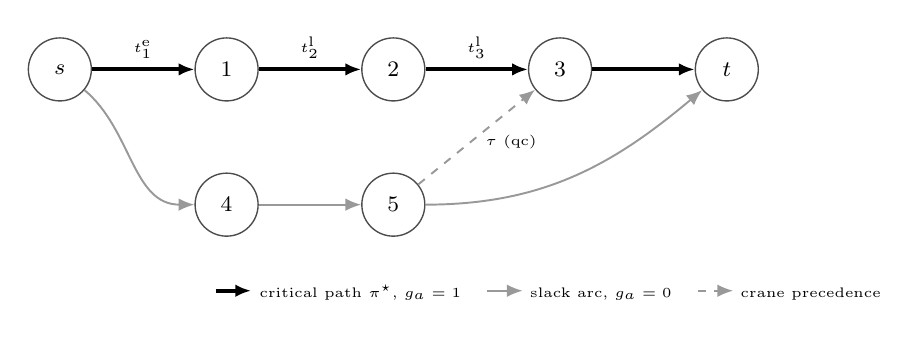
\begin{tikzpicture}[node distance=8mm and 13mm]
% --- the two vehicle chains, drawn as one row each so no arc crosses a node -------------
\node[ev] (s) {$s$};
\node[ev, right=of s]  (a1) {$1$};
\node[ev, right=of a1] (a2) {$2$};
\node[ev, right=of a2] (a3) {$3$};
\node[ev, right=of a3] (t)  {$t$};
\node[ev, below=9mm of a1] (b1) {$4$};
\node[ev, right=of b1]     (b2) {$5$};

% vehicle chain 1 -- critical
\draw[fl, crit] (s)--(a1)  node[midway, above, font=\tiny] {$t^{\mathrm e}_1$};
\draw[fl, crit] (a1)--(a2) node[midway, above, font=\tiny] {$t^{\mathrm l}_2$};
\draw[fl, crit] (a2)--(a3) node[midway, above, font=\tiny] {$t^{\mathrm l}_3$};
\draw[fl, crit] (a3)--(t);
% vehicle chain 2 -- slack
\draw[fl, slack] (s)  to[out=-40, in=180] (b1);
\draw[fl, slack] (b1)--(b2);
\draw[fl, slack] (b2) to[out=0, in=-140] (t);
% crane serialisation arc, entering node 3 from below so it crosses nothing
\draw[fl, dashed, slack] (b2)--(a3)
  node[pos=0.45, right=0.6mm, font=\tiny] {$\tau$ (qc)};

% --- key, placed beneath the graph rather than floating beside it ----------------------
\node[font=\tiny, anchor=north west, align=left] at ([yshift=-6mm]b1.south west)
  {\tikz{\draw[fl,crit]  (0,0)--(4.5mm,0);}~critical path $\pi^\star$, $g_a = 1$ \quad
   \tikz{\draw[fl,slack] (0,0)--(4.5mm,0);}~slack arc, $g_a = 0$ \quad
   \tikz{\draw[fl,dashed,slack] (0,0)--(4.5mm,0);}~crane precedence};
\end{tikzpicture}
\caption[The event DAG of a small schedule]{The event DAG of a small schedule. Solid arcs are vehicle legs and the dashed arc a
quay-crane serialisation constraint. The bold path $s \to 1 \to 2 \to 3 \to t$ is the critical
path $\pi^\star$; by Section~\ref{sec:maxplus} only its arcs carry a non-zero attribution, and
their durations sum to $\Cmax$ by Eq.~\eqref{eq:decomposition}.}
\label{fig:dag}
\end{figure}

\section{The multi-population biased random-key genetic algorithm}
\label{sec:mpbrkga}

Fronts are produced by the mp-BRKGA of \citet{fontes2023}, reimplemented against the authors'
own solver source. The reimplementation was diffed against that source operator by operator
before any result was produced, and the correspondence is stated exactly rather than assumed. The
objective is identical, not approximately so: his is split across a per-task completion array and
a per-vehicle availability array, ours takes a single maximum over completions, and the asymmetry
of~\eqref{eq:load} and~\eqref{eq:unload} makes the two equal, which
Chapter~\ref{sec:evaluation} confirms on 2400 random schedules at exactly zero difference. The
elite and mutant counts use his \texttt{ceil} rounding, and the second crossover parent is drawn
from the non-elites as in his disjoint parent ranges. One representational difference remains:
his mutants store integer speed and vehicle indices directly in blocks two to four, whereas ours
stores random keys that the decoder buckets into the same levels. The induced distribution over
decoded mutants is therefore the same, and was checked to be so, but the chromosome encoding
differs and a seed-for-seed reproduction of his trajectory is not possible. Following the biased random-key paradigm \citep{goncalves2011} a solution is
a vector of $4N$ keys, one block of task priorities, two of empty- and loaded-leg speed levels
and one of vehicle assignments, which a decoder maps to a schedule that is then evaluated
exactly. The method evolves $\Omega + \Pi$ populations concurrently: each single-objective
population ranks by one objective and so drives one extreme of the front, while each
multi-objective population ranks by non-dominated sorting with crowding distance
\citep{deb2002}. Each generation replaces a population by its elite fraction, offspring from
biased parameterised uniform crossover inheriting from the elite parent with probability
$p_e = 0.7$, and fresh mutants; elites migrate between populations so that boundary specialists
propagate inward.

The published configuration is $P = 20N$ per population, elite fraction $0.2$, mutant fraction
$0.1$, $p_e = 0.7$, $\Omega = \Pi = 2$ and $n_{ex} = 30$, adopted here with the reduced
generation budget of Section~\ref{sec:design}. The search is not a contribution of this work; it
is the instrument supplying Pareto-optimal schedules to be explained, and no learned model
participates in producing any front reported here.

\section{Selection of the surrogate model class}
\label{sec:whygnn}

Exact evaluation costs well under a millisecond at these sizes, so a surrogate is not required to
render search tractable. Its purpose is that a model predicting the per-activity structure of a
schedule can be differentiated with respect to its own predictions, yielding an explanation
derived from a learned representation rather than from the exact recurrence, which the two can
then be compared on. Establishing that the explanation is learnable is a precondition for any
setting in which the exact recurrence is unavailable.

Three properties of the input determine the model class. First, a resolved schedule is a typed
precedence graph, not a vector. Any model consuming a fixed-length feature vector must serialise
it as the $4N$ chromosome of Section~\ref{sec:mpbrkga}, as a tree ensemble such as XGBoost
\citep{chen2016} would; that representation has a length depending on $N$, so it does not
transfer across instance sizes, and its coordinates are decision-variable indices, so any
attribution over it, TreeSHAP \citep{lundberg2020} included, attributes to chromosome positions
rather than to physical activities. Second, the recurrences
\eqref{eq:load}--\eqref{eq:unload} relate a task to its immediate predecessor on a resource,
which is message passing \citep{gilmer2017}: a graph network is constrained to the locality a
multilayer perceptron would have to learn. Third, the two relations enter \eqref{eq:load} and
\eqref{eq:unload} differently and therefore cannot share parameters, and the quantities that
matter, travel time and leg energy, are properties of arcs rather than nodes, which forces edge
conditioning.

These jointly specify a heterogeneous, edge-conditioned message-passing network. The attentional
variant is adopted in the corrected GATv2 form of \citet{brody2022} rather than the original GAT
\citep{velickovic2018}, whose attention is monotonic in the key and therefore cannot rank
neighbours conditioned on the query. Cross-relation fusion follows the semantic attention of
\citet{wang2019han}; Section~\ref{sec:arch} explains why that cross-relation attention, and not
the within-relation attention, carries the informative signal here.

% ======================================================================================
\chapter{Method and Experimental Design}
\label{sec:method}

\section{Research question}

The investigation asks whether, for a schedule on the Pareto front of the problem of
Chapter~\ref{sec:motivation}, one can state exactly why it is efficient, and whether that
explanation varies systematically along the front. The first part is addressed constructively by
the architecture below; the second is empirical and requires a scalar summary of an explanation.

\section{Graph representation}
\label{sec:graph}

Figure~\ref{fig:pipeline} gives the pipeline as a whole; this subsection and the two that follow
describe its three stages.

\begin{figure}[tb]
\centering
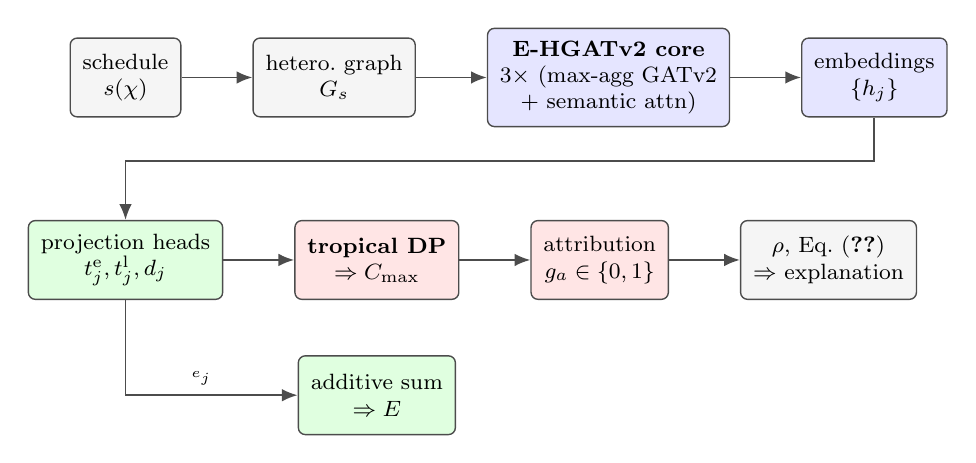
\begin{tikzpicture}[node distance=6mm and 9mm]
\node[io]                   (sched) {schedule\\$s(\chi)$};
\node[io,   right=of sched] (graph) {hetero.\ graph\\$G_s$};
\node[core, right=of graph] (core)  {\textbf{E-HGATv2 core}\\$3\times$ (max-agg GATv2\\$+$ semantic attn)};
\node[core, right=of core]  (emb)   {embeddings\\$\{h_j\}$};

\node[head, below=13mm of sched] (proj) {projection heads\\$t^{\mathrm e}_j, t^{\mathrm l}_j, d_j$};
\node[dp,   right=of proj]       (dpn)  {\textbf{tropical DP}\\$\Rightarrow \Cmax$};
\node[dp,   right=of dpn]        (tape) {attribution\\$g_a \in \{0,1\}$};
\node[io,   right=of tape]       (rho)  {$\rho$, Eq.~\eqref{eq:rho}\\$\Rightarrow$ explanation};
\node[head, below=7mm of dpn]    (en)   {additive sum\\$\Rightarrow E$};

\draw[fl] (sched)--(graph);
\draw[fl] (graph)--(core);
\draw[fl] (core)--(emb);
\draw[fl] (emb.south) -- ++(0,-5.5mm) -| (proj.north);
\draw[fl] (proj)--(dpn);
\draw[fl] (dpn)--(tape);
\draw[fl] (tape)--(rho);
\draw[fl] (proj.south) |- (en.west) node[pos=0.72, above, font=\tiny] {$e_j$};
\end{tikzpicture}
\caption[The E-HGATv2 pipeline]{The pipeline. The core embeds a decoded schedule; projection heads
predict \emph{local physical attributes}, which an exact max-plus dynamic programme composes into
$\Cmax$, energy being an exact additive sum. Differentiating the dynamic programme yields the
binary attributions $g_a = \partial\Cmax/\partial w_a$, from which $\rho$ is computed. The network
never regresses an objective directly.}
\label{fig:pipeline}
\end{figure}

A resolved schedule is encoded as a heterogeneous graph. Nodes are tasks, carrying four features:
the handling time $\tau_j$, two indicators distinguishing loading from unloading, and the
identifier of the servicing crane. Arcs are of two types. An \emph{AGV arc} connects consecutive
tasks on the same vehicle; a \emph{QC arc} connects consecutive tasks on the same crane. Each arc
carries three features: the total travel time of the leg it represents and the empty and loaded
energies of that leg.

The graph is therefore precisely the precedence DAG of Figure~\ref{fig:dag}, so the
representation is isomorphic to the combinatorial structure of the objective. Two aspects are
consequential: each task has at most one incoming arc of each type, with the architectural
implication of Section~\ref{sec:arch}, and travel time and energy reside on arcs, so the model
must condition its messages on edge attributes rather than on node states alone.

\section{The E-HGATv2 architecture}
\label{sec:arch}

Each layer updates the fixed-length description held at every task by combining it with those
held at its immediate predecessors on its vehicle and on its crane, so stacking $L$ layers lets
information reach a task from predecessors up to $L$ positions away in either chain. The
surrogate has three such layers, a hidden dimension of $64$ and four attention heads per layer,
and each layer performs two operations.

\paragraph{Within-relation propagation under a max-plus reduction.} For each relation
$R \in \{\text{AGV}, \text{QC}\}$ separately, a GATv2 convolution \citep{brody2022} conditioned
on the arc attributes computes a message for every node from its predecessors under $R$. The
aggregation is \texttt{max} rather than the customary attention-weighted sum. This choice mirrors
the semiring: the recurrences of Section~\ref{sec:maxplus} reduce a node's same-resource
predecessors under a maximum, and the aggregator is therefore selected to match the algebra of
the problem rather than for its smoothness.

\paragraph{Cross-relation fusion by semantic attention.} The two relation messages are combined
by a learned attention over relations, in the manner of \citet{wang2019han}. This is where the
informative signal resides, and the reason is a direct consequence of the encoding of
Section~\ref{sec:graph}. Since a resolved schedule gives each task at most one predecessor per
resource, the within-relation attention softmax is computed over a single incoming arc and is
therefore degenerate, equal to one identically. It contributes no discriminative information.
The non-degenerate quantity is which of the two resources gates the task, exactly the
$\max(\text{agv\_ready}, \text{qc\_ready})$ argmax of the recurrence, and this is what the
cross-relation attention represents. Its per-node weight on a relation is interpretable as the
criticality of the corresponding incoming arc, and it is recorded per arc for that purpose.

This asymmetry inverts the conventional reading of an attentional graph network, in which the
within-neighbourhood attention constitutes the object of interest. In the present setting that
component is structurally vacuous, and the cross-relation component carries the resource-contention
signal. Figure~\ref{fig:layer} shows one layer.

\begin{figure}[!htb]
\centering
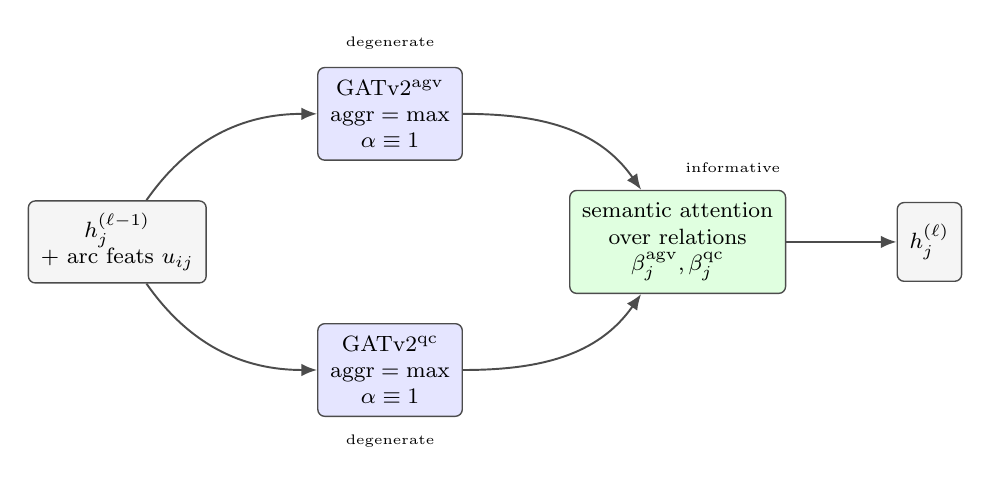
\begin{tikzpicture}[node distance=7mm and 14mm]
\node[io] (hin) {$h^{(\ell-1)}_j$\\$+$ arc feats $u_{ij}$};
\node[core, above right=5mm and 14mm of hin] (agv)
  {GATv2$^{\mathrm{agv}}$\\$\mathrm{aggr}=\max$\\$\alpha \equiv 1$};
\node[core, below right=5mm and 14mm of hin] (qc)
  {GATv2$^{\mathrm{qc}}$\\$\mathrm{aggr}=\max$\\$\alpha \equiv 1$};
\node[head, right=14mm of hin, xshift=32mm] (sem)
  {semantic attention\\over relations\\$\beta^{\mathrm{agv}}_j, \beta^{\mathrm{qc}}_j$};
\node[io, right=of sem] (hout) {$h^{(\ell)}_j$};
\draw[fl] (hin) to[out=55,  in=180] (agv);
\draw[fl] (hin) to[out=-55, in=180] (qc);
\draw[fl] (agv) to[out=0, in=125] (sem);
\draw[fl] (qc)  to[out=0, in=-125] (sem);
\draw[fl] (sem)--(hout);
\node[font=\tiny, above=1mm of agv] {degenerate};
\node[font=\tiny, below=1mm of qc]  {degenerate};
\node[font=\tiny, above=1mm of sem, xshift=7mm] {informative};
\end{tikzpicture}
\caption[One heterogeneous layer]{One heterogeneous layer. Message passing runs independently per
relation under a maximum aggregation, and the two relation messages are then fused by a learned
attention across relations. Within a relation a resolved schedule gives each task at most one
incoming arc, so the GATv2 softmax is over a single arc and is degenerate ($\alpha \equiv 1$).
Across relations $\beta_j$ is non-degenerate and encodes which resource gates task $j$, the
$\max(\text{agv\_ready}, \text{qc\_ready})$ argmax of the recurrence; it is recorded per arc as
that arc's criticality. The informative attention is therefore the cross-relation one.}
\label{fig:layer}
\end{figure}

\section{The tropical max-plus layer}
\label{sec:tropical}

The architecture described so far could be completed in the conventional manner, by pooling node
embeddings and regressing $(\Cmax, E)$ with a multilayer perceptron. Doing so defeats the purpose
of the exercise. A pooled regression head mixes every node embedding into every output, so the
Jacobian of the predicted makespan with respect to the input features is dense. An attribution
read from it distributes credit across activities that are provably irrelevant, because
Section~\ref{sec:maxplus} establishes that only the activities of one path can affect $\Cmax$ at
all. The head, not the encoder, is what destroys faithfulness.

The makespan head is therefore replaced by a differentiable max-plus dynamic programme. The layer
computes, for a directed acyclic graph of activity events,
\begin{equation}
x[v] = w[v] + \max_{u \to v}\bigl(x[u] + w[u,v]\bigr),
\label{eq:tropical}
\end{equation}
in a deterministic topological order obtained by Kahn's algorithm, with node weights $w[v]$ and
edge weights $w[u,v]$ supplied by the network. The makespan is the maximum over sinks. The layer
is implemented as a custom autograd operation: the forward pass records the maximising predecessor
of each node, and the backward pass routes the incoming subgradient exclusively through that
recorded argmax edge.

The consequence is the property sought. Because the backward pass follows a single path,
$\partial \Cmax / \partial(\text{activity duration})$ is exactly one for activities on the
critical path and exactly zero otherwise. Attribution is not estimated; it is read off a
selection that the forward pass already made. Figure~\ref{fig:autograd} contrasts this with the
pooled head it replaces.

\begin{figure}[tb]
\centering
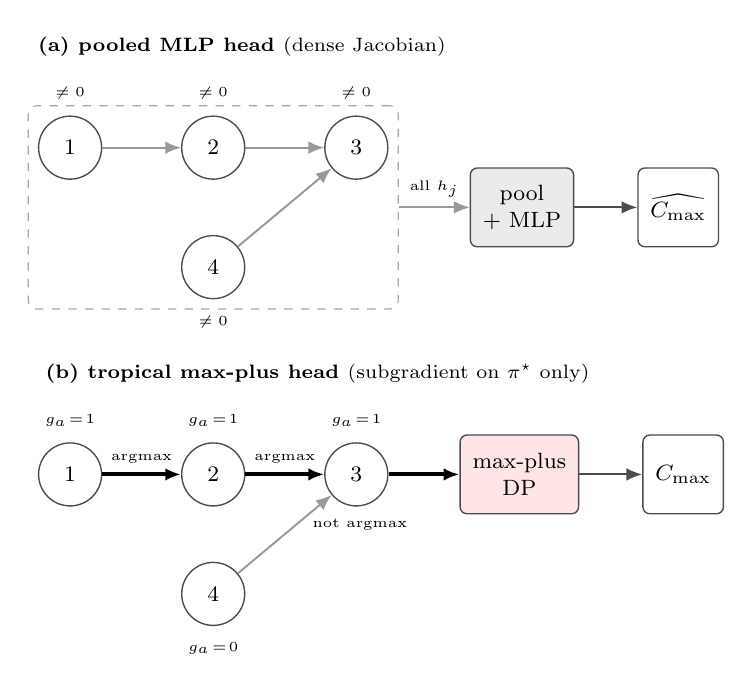
\begin{tikzpicture}[node distance=7mm and 10mm]
\begin{scope}[local bounding box=panA]
  \node[ev] (p1) {$1$};
  \node[ev, right=of p1] (p2) {$2$};
  \node[ev, right=of p2] (p3) {$3$};
  \node[ev, below=7mm of p2] (p4) {$4$};
  \draw[fl, slack] (p1)--(p2);
  \draw[fl, slack] (p2)--(p3);
  \draw[fl, slack] (p4)--(p3);
  \node[draw=black!35, dashed, rounded corners=3pt, inner sep=3.5pt,
        fit=(p1)(p2)(p3)(p4)] (fitA) {};
  \node[blk, fill=black!8, right=9mm of fitA] (pool) {pool\\$+$ MLP};
  \node[blk, right=8mm of pool] (out1) {$\widehat{\Cmax}$};
  \draw[fl, slack] (fitA)--(pool) node[midway, above, font=\tiny] {all $h_j$};
  \draw[fl] (pool)--(out1);
  \foreach \n in {p1,p2,p3} \node[font=\tiny, above=0.8mm of \n] {$\neq 0$};
  \node[font=\tiny, below=0.8mm of p4] {$\neq 0$};
\end{scope}
\node[font=\scriptsize\bfseries, anchor=south west] at ([yshift=1.5mm]panA.north west)
  {(a) pooled MLP head \textnormal{(dense Jacobian)}};

\begin{scope}[shift={(0,-4.15)}, local bounding box=panB]
  \node[ev] (q1) {$1$};
  \node[ev, right=of q1] (q2) {$2$};
  \node[ev, right=of q2] (q3) {$3$};
  \node[ev, below=7mm of q2] (q4) {$4$};
  \draw[fl, crit]  (q1)--(q2) node[midway, above, font=\tiny] {argmax};
  \draw[fl, crit]  (q2)--(q3) node[midway, above, font=\tiny] {argmax};
  \draw[fl, slack] (q4)--(q3) node[pos=0.62, right=0.8mm, font=\tiny] {not argmax};
  \node[dp, right=9mm of q3] (dpb) {max-plus\\DP};
  \node[blk, right=8mm of dpb] (out2) {$\Cmax$};
  \draw[fl, crit] (q3)--(dpb);
  \draw[fl] (dpb)--(out2);
  \foreach \n in {q1,q2,q3} \node[font=\tiny, above=0.8mm of \n] {$g_a\!=\!1$};
  \node[font=\tiny, below=0.8mm of q4] {$g_a\!=\!0$};
\end{scope}
\node[font=\scriptsize\bfseries, anchor=south west] at ([yshift=1.5mm]panB.north west)
  {(b) tropical max-plus head \textnormal{(subgradient on $\pi^\star$ only)}};
\end{tikzpicture}
\caption[Pooled regression head against the tropical head]{The output head, not the encoder,
determines whether the attribution is faithful. Both panels encode the same four activities, three
on the longest path while activity $4$ loses the maximum at node $3$. (a) A pooled regression head
mixes every node embedding into the output, so every activity receives a non-zero derivative,
including activity $4$, which provably cannot affect $\Cmax$. (b) The max-plus layer records the
maximising predecessor during the forward pass and routes the subgradient through it alone, so the
attribution is the indicator of the critical path.}
\label{fig:autograd}
\end{figure}

Equation~\eqref{eq:decomposition} then holds for
the model's own predicted durations exactly as it holds for the exact ones, which is what permits
the model's explanation and the exact explanation to be compared on identical terms. The layer
belongs to the family of differentiable optimisation layers \citep{amos2017, pogancic2020}, and
is distinguished by the fact that the embedded computation is a dynamic programme whose
subgradient is available in closed form rather than an optimisation requiring implicit
differentiation.

Ties in~\eqref{eq:tropical} are resolved by the first maximum in edge order, following the
deterministic \texttt{argmax} convention. This is a valid subgradient selection, since any single
maximiser of a maximum is a subgradient; Chapter~\ref{sec:limitations} reports a defect arising
where the surrounding analysis code does not respect this convention.

\paragraph{Prediction targets, anchoring and the energy head.} The network does not predict the
objectives. An arc-level head maps the concatenated endpoint embeddings of a task's incoming AGV
arc to its empty and loaded travel times and leg energies, and a node-level head maps a task
embedding to its crane handling delay; the makespan is composed from these
by~\eqref{eq:tropical} and the energy by exact summation, a linear head for which
$\partial E / \partial e_\ell = 1$ identically. Because a max-plus output constrains only the
attributes on the currently active path, training on the makespan alone would leave off-path
attributes unidentified, so the local attributes are supervised directly against their exact
physical values. Training is therefore two-stage rather than end-to-end: the core is trained
first, then frozen with cached embeddings while the heads are fitted. One consequence should be
read with care. The arc features the encoder aggregates include the per-leg energies themselves,
so predicting total energy is close to reading a sum of inputs, and the near-unit coefficient of
determination in Section~\ref{sec:surrogate-eval} is a property of the architecture rather than
evidence of learning.

\section{The duration-weighted critical share}
\label{sec:rho}

Comparing explanations across schedules requires a scalar. The natural candidate is the
proportion of the critical path attributable to vehicle travel rather than crane handling.

Counting on-path activities of each kind is inadequate. Legs and handlings are not
commensurable: a task may contribute a critical handling while its vehicle
chain also binds, so the two counts neither partition the path nor sum to a meaningful total. An
earlier formulation of this work used counting and produced a measure that failed to reconcile
with the makespan.

The measure adopted here weights by duration. Define
\begin{equation}
\rho_{\text{transport}} =
\frac{\sum_{\text{on-path legs}} d_\ell}
     {\sum_{\text{on-path legs}} d_\ell + \sum_{\text{on-path tasks}} \tau_j},
\qquad
\rho_{\text{handling}} = 1 - \rho_{\text{transport}}.
\label{eq:rho}
\end{equation}
By~\eqref{eq:decomposition} the denominator equals $\Cmax$ exactly, so the two shares partition
the makespan and sum to unity by construction. Neither term counts objects, which removes the
commensurability problem entirely.

The quantity of interest is the shift in $\rho_{\text{transport}}$ between the two ends of the
front,
\begin{equation}
\text{migration} = \rho_{\text{transport}}(\text{makespan-optimal})
                 - \rho_{\text{transport}}(\text{energy-optimal}).
\label{eq:migration}
\end{equation}
The sign is retained rather than taken in absolute value, because it identifies which end is
travel-heavy. A negative value indicates that the energy-optimal end leans more on travel than the
makespan-optimal end does, so that prioritising energy moves the bottleneck towards vehicle
travel; a positive value indicates the converse; and a value near zero indicates that the character
of the bottleneck is invariant along the front even though the objective values are not.

\section{Experimental design}
\label{sec:design}

\paragraph{Instances.} Two published sets are used directly \citep{fontes2022, fontes2023}, and
a further two families are constructed from the first as Section~\ref{sec:families} describes.
The small set comprises 35 loading instances of 4 to 16 tasks on a six-crane, six-station layout. The large
dual-cycling set comprises 10 instances of 40 to 160 tasks on a twenty-crane, twenty-station
layout; it is referred to throughout as the large dual-cycling set, to distinguish it from the
26 small mixed instances of Section~\ref{sec:families}, which are dual-cycling in the same
operational sense but are a different set on a different layout.
Both were transcribed programmatically from the published tables and the authors' solver
sources; no value was retyped. The transcription was cross-validated: the distance matrix and
task lists were parsed independently twice and agreed in every cell, and four published optima
and five mixed-instance pairings matched exactly.

\paragraph{Fleet sweep.} The parameter of interest is the fleet-to-crane ratio $A/Q$. Because
every published large instance has $A/Q = 0.50$, the published sets cannot by themselves
determine whether migration depends on this ratio. Six small instances (L01, L07, L15, L21, L28,
L35) were therefore each run at nine fleet sizes, $A \in \{1,\dots,9\}$, with ten seeds: 540
replicates, all other parameters fixed.

\paragraph{Front campaign.} The sweep above varies the ratio on six loading instances and records
the transport share at the two extremes of each front. A second campaign widens both axes. It
covers all 96 instances of the three families of Section~\ref{sec:families} at the same nine
fleet sizes and ten seeds, giving 8{,}640 replicates, and computes the share at every point of
every front rather than at its extremes, giving 657{,}899 explained schedules. No surrogate is
fitted in this campaign: every quantity is produced by the exact evaluator and the exact
attribution, so a replicate costs a few seconds and the whole campaign runs in about ten minutes
on 200 cores.

\paragraph{Budget and statistics.} Each replicate runs mp-BRKGA at $P = 20N$ per population with
$\Omega = \Pi = 2$, $n_{ex} = 30$ and 100 generations, below the published $300$; since no
comparison is against a published front and every arm shares the budget, the reduction affects
absolute front quality but not the migration measurement. Migration is tested against zero by a
one-sample Wilcoxon signed-rank test across the ten seeds of each instance--fleet cell, with
$p$-values Holm-corrected \citep{holm1979} within each instance's nine fleet sizes so that nine
simultaneous tests cannot produce a spurious rejection. Effect size is the matched-pairs
rank-biserial correlation \citep{kerby2014}. A non-parametric procedure is used because ten
observations per cell do not support a distributional assumption and several cells are degenerate
with near-zero variance. Front quality, where reported, uses hypervolume \citep{zitzler1999} and
IGD$^+$ \citep{ishibuchi2015}.

\section{Software architecture and implementation}
\label{sec:software}

The implementation is a Python package of 50 modules and approximately 10{,}200 source lines,
organised so that the exact physics, the learned model and the search are separable and
independently testable. The \texttt{environment} package is the exact physics and carries no
learned component; \texttt{surrogate} holds the graph construction and the encoder;
\texttt{explain} holds the tropical layer, the fused head and both explainers; and
\texttt{baselines}, \texttt{metrics} and \texttt{benchmark} form the evaluation harness.



\paragraph{The exact evaluator as label source.} There is no external dataset. Every training
target is produced by the exact evaluator, which runs \eqref{eq:load}--\eqref{eq:cmax} in
topological order in $O(N)$ and returns both the objective pair and the per-task quantities the
projection heads are supervised on. Random-key vectors are sampled uniformly, decoded and
evaluated, so the data is generated self-supervised. This is what makes the physics anchoring of
Section~\ref{sec:tropical} possible, and it is why the evaluator's agreement with the source work
is a precondition for every other result.

\paragraph{The autograd function.} The max-plus layer is a \texttt{torch.autograd.Function}
rather than a composition of differentiable primitives, because the required backward behaviour is
not the one automatic differentiation would supply for a chain of \texttt{torch.maximum} calls.
The forward pass establishes a deterministic topological order by Kahn's algorithm, rejecting
any input that is not acyclic, since the precedence graph of a feasible schedule must be a DAG. It
then relaxes~\eqref{eq:tropical} in that order, and stores the maximising predecessor of every node.
The backward pass then walks the stored selections in reverse, accumulating the incoming
gradient into exactly one predecessor per node. The \texttt{argmax} used in the forward pass is
what implements the tie convention: it returns the first maximal index, so a tie yields one valid
subgradient rather than a blend of several.

Chapter~\ref{sec:limitations} records a case in which downstream analysis code violated this
convention and the decomposition consequently failed to close.

\paragraph{Assertions, testing and execution.} Node and arc feature tensors are validated at
every entry point against declared semantic signatures, and the decomposition
identity~\eqref{eq:decomposition} is asserted on every traversal at a relative tolerance of
$10^{-6}$, so an inconsistency raises rather than being averaged into a table. The suite comprises
29 unit-test modules and 239 tests, all passing, including the equivalence of the max-plus
evaluator with an exhaustive enumeration of all 1248 schedule structures on a five-task instance
and the mp-BRKGA operator semantics against the authors' source. Campaigns ran on a rented cloud
instance of 384 vCPU and 125\,GB RAM under Python 3.12 and PyTorch 2.11, distributed over a
process pool; the 540-replicate sweep took 47 minutes and the 350-replicate small-set campaign 10
minutes, neither with a single failure.

\section{Reproducibility}

Every table in Chapter~\ref{sec:evaluation} is generated programmatically from the stored
experiment output, so no figure in this document is transcribed by hand. Replicates are seeded
and isolated: a failure in one cannot affect another, and failures are counted in the output.
Every replicate of every campaign ran to completion: no run crashed, timed out or was lost, over
the 940 replicates of the sweeps and the 8{,}640 of the front campaign alike. The decomposition
check of Chapter~\ref{sec:limitations} is satisfied as widely: the recovered critical path
reconciles with the makespan on all 940 replicates and at all 657{,}899 front points, so no
quantity reported in this document is computed on a filtered subset. An earlier version of the
attribution failed that check on a small fraction of cases; the defect, its diagnosis and its
correction are reported in Chapter~\ref{sec:limitations}.

% ======================================================================================
\chapter{Results}
\label{sec:evaluation}

\section{Verification against the source work}

Before any explanation may be trusted the evaluator must agree with the source work.
\citet{fontes2023} compute the objective as $\max(\max_j c_j,\ \max_a A_a)$, in which $A_a$ tracks
when vehicle $a$ next becomes available, whereas the implementation here takes a single maximum
over per-task completions. The expressions are identical, and the reason is the asymmetry
of~\eqref{eq:load} and~\eqref{eq:unload}: for a LOAD the availability equals $c_j - \tau_j$, the
vehicle being released as soon as the crane assumes the container, and is dominated by
$\max_j c_j$; for an UNLOAD it equals the completion of the loaded leg, which
by~\eqref{eq:unload} is exactly $c_j$. The reference implementation distributes across two arrays
what~\eqref{eq:cmax} folds into one. On 2400 random schedules across eight instances of both sets
the two expressions agreed to exactly zero difference in every case.

A second, independent check compares the makespan-optimal end of the computed fronts against the
mixed-integer optima published for all 35 small instances \citep{fontes2022}. This is not a test
of exact agreement: the published optima are computed for fixed-speed scenarios, whereas the
present runs select among three speeds per leg and therefore solve a less constrained problem
whose makespan should lie at or below any fixed-speed optimum. A value above one would indicate
an evaluator error or a search shortfall; a value below is the expected consequence of the
enlarged decision space.

Table~\ref{tab:published} reports the comparison. Across all four published makespan columns
the best computed makespan lies at or below the published value in effectively every comparable
cell, the two exceptions being L03 and L25, which exceed the nominal-higher column by $0.56$ and
$1.56$ seconds respectively.

% ---- BEGIN generated: tables/published.tex (scripts/make_thesis_tables.py) ----
% Generated by scripts/make_thesis_tables.py -- do not edit by hand.
\begin{table}[tb]
\centering
\small
\caption[Computed fronts against the published fixed-speed optima]{The makespan-optimal end of the computed fronts against the published fixed-speed optima, over the 35 small instances. The present runs select among three speeds per leg and therefore solve a less constrained problem, so the computed value should lie at or below each published optimum; a value above one would indicate an evaluator error or a search shortfall. The nominal--higher scenario is the nearest comparison because it permits the highest fixed speed. 14 published cells are blank, the authors' solver having failed to close them, and are skipped rather than imputed.}
\label{tab:published}
\footnotesize
\begin{tabular}{lrrrr}
\toprule
Published column & comparable & at or below & exact & mean gap (s) \\
\midrule
nominal, $C_{\max}$ & 35 & 35 & 0 & $-365.75$ \\
nominal, $C_{\max}^{\star}$ & 35 & 35 & 0 & $-98.69$ \\
lower--nominal, $C_{\max}$ & 33 & 33 & 0 & $-530.13$ \\
nominal--higher, $C_{\max}^{\star}$ & 23 & 21 & 1 & $-17.26$ \\
\bottomrule
\end{tabular}
\end{table}
% ---- END generated: tables/published.tex ----

The loading family is Table~5 as printed, but the unloading and mixed families are reconstructions, so each is checked against the optima published for it.
Table~\ref{tab:validation} reports both.

% ---- BEGIN generated: tables/validation.tex (scripts/make_thesis_tables.py) ----
% Generated by scripts/make_thesis_tables.py -- do not edit by hand.
\begin{table}[tb]
\centering
\small
\caption[Reconstructed families against the published optima]{The two reconstructed instance families against the mixed-integer optima published for them, at the published fleet size of two vehicles. The unloading family reverses the origins and destinations of Table~5; the mixed family combines the pairs named in the ``comb.\ of'' column of Table~3, and is the 26-instance small set, not the ten large dual-cycling instances of Table~\ref{tab:dl}. Ratios below one are expected, since the runs here select among three speeds per leg where the published optima fix one, so they solve a less constrained problem. The final column counts instances whose energy optimum is reproduced exactly, which the speed selection cannot improve upon and which therefore tests the reconstruction directly.}
\label{tab:validation}
\footnotesize
\begin{tabular}{lrrrrr}
\toprule
Family & instances & \multicolumn{2}{c}{$C_{\max}$ ratio} & $E$ ratio & $E$ exact \\
\cmidrule(lr){3-4}\cmidrule(lr){5-5}\cmidrule(l){6-6}
 & & mean & range & mean & \\
\midrule
unloading & 35 & 0.915 & 0.740--0.975 & 0.996 & 18/33 \\
mixed & 26 & 0.935 & 0.793--1.030 & 0.960 & 11/25 \\
\bottomrule
\end{tabular}
\end{table}
% ---- END generated: tables/validation.tex ----


The closest correspondence is with the normal-higher scenario, at a mean gap of $-17.26$ seconds,
and on L01 the agreement is exact: the makespan-optimal end is $175.00$ against a published
$175$. That this is the nearest column is the expected outcome, since that scenario permits the
highest fixed speed and is therefore the fixed-speed problem closest to the present one. The
check establishes that the evaluator operates in the correct regime and never produces an
implausibly low makespan against an independently computed bound; it does not, and cannot,
reproduce the published values.

\section{A worked example}

Table~\ref{tab:traversal} presents the complete exact explanation of a single schedule: the
makespan-optimal Pareto point of L01, the smallest instance and therefore verifiable by hand. The
critical path comprises five activities whose durations sum to the makespan exactly,
as~\eqref{eq:decomposition} requires.

% ---- BEGIN generated: tables/traversal.tex (scripts/make_thesis_tables.py) ----
% Generated by scripts/make_thesis_tables.py -- do not edit by hand.
\begin{table}[tb]
\centering
\small
\caption[Worked example: the exact critical path of L01]{Worked example: the exact makespan critical path of the makespan-optimal Pareto schedule of L01 ($N=4$, $A=2$, $Q=2$). The on-path durations sum to $C_{\max} = 175.000$ exactly, because every on-path activity carries a unit subgradient. No surrogate is involved in producing this table.}
\label{tab:traversal}
\footnotesize
\begin{tabular}{rllrrl}
\toprule
Order & Task & Activity & Duration (s) & $\partial C_{\max}$ & Resource \\
\midrule
0 & $t_{2}$ & empty\_leg & 0.000 & 1 & AGV~1, QC2 \\
1 & $t_{2}$ & loaded\_leg & 55.556 & 1 & AGV~1, QC2 \\
2 & $t_{1}$ & empty\_leg & 27.778 & 1 & AGV~1, QC1 \\
3 & $t_{1}$ & loaded\_leg & 41.667 & 1 & AGV~1, QC1 \\
4 & $t_{1}$ & qc\_handling & 50.000 & 1 & AGV~1, QC1 \\
\midrule
\multicolumn{3}{l}{Sum of on-path durations} & 175.000 & & $= C_{\max}$ \\
\multicolumn{3}{l}{of which travel / handling} & 125.000 / 50.000 & & $\rho = 0.714$ \\
\bottomrule
\end{tabular}
\end{table}
% ---- END generated: tables/traversal.tex ----

Two properties of this traversal are of note. Every on-path activity belongs to the same vehicle,
which establishes that the schedule is vehicle-limited and that the pertinent intervention is
fleet capacity rather than crane rebalancing. The division between travel and handling is
quantified rather than asserted: $\rho = 0.714$ indicates that slightly over seventy per cent of
the makespan consists of vehicle movement and the remainder of crane handling. This constitutes
the form of statement the thesis set out to produce.

\begin{figure}[tb]
\centering
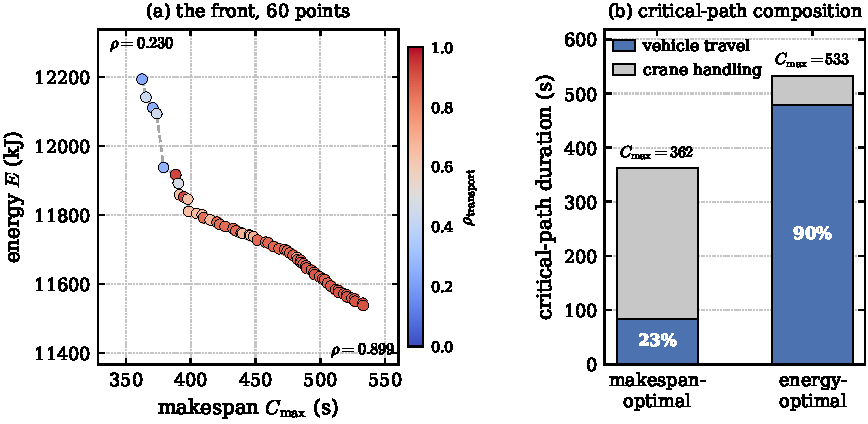
\includegraphics[width=0.78\textwidth]{figs/fig_front.pdf}
\caption[One explained front]{One explained front, for L21 at $A/Q = 1.67$ and seed $0$, whose ten-seed cell mean
appears in Table~\ref{tab:migration}. (a) All sixty non-dominated points on the objective
plane, each shaded by its duration-weighted transport share, so that the figure reports not
only the trade-off but what binds at each compromise. The makespan-optimal end is crane-bound
($\rho_{\text{transport}} = 0.230$) and the energy-optimal end vehicle-bound
($\rho_{\text{transport}} = 0.899$); the transition between them occurs across the front rather
than at its ends. (b) The critical path of each extreme resolved into its travel and handling
parts, which sum to that end's makespan by Eq.~\eqref{eq:decomposition}. The share, not the
objective value, is what the explanation reports.}
\label{fig:front}
\end{figure}

\section{The degenerate regime}
\label{sec:degenerate}

Table~\ref{tab:dl} applies the method to both front extremes of all ten large dual-cycling
instances, at up to 160 tasks. The decomposition closes on all 50 replicates.

% ---- BEGIN generated: tables/dl.tex (scripts/make_thesis_tables.py) ----
% Generated by scripts/make_thesis_tables.py -- do not edit by hand.
\begin{table}[tb]
\centering
\small
\caption[Exact explanation of both front extremes on the dual-cycling set]{Exact explanation of both front extremes on the ten large dual-cycling instances, averaged over five seeds each. Every instance has $A/Q = 0.50$, and the transport share is high at both ends, so migration is negligible throughout. Migration is the makespan-optimal share minus the energy-optimal share, as in Table~\ref{tab:migration}. This is the degenerate regime that motivates the sweep in Table~\ref{tab:migration}. The final two columns are the learned surrogate's own migration on the same fronts and the Jaccard agreement of its recovered critical leg set with the exact one, so the model is measured on the largest instances in the study rather than only on the small ones. The decomposition closes on all 50 replicates, so none is excluded.}
\label{tab:dl}
\footnotesize
\begin{tabular}{lrrrrrrrrr}
\toprule
& & & & \multicolumn{2}{c}{exact} & \multicolumn{2}{c}{exact share} & \multicolumn{2}{c}{surrogate} \\
\cmidrule(lr){5-6}\cmidrule(lr){7-8}\cmidrule(l){9-10}
Instance & $N$ & $A/Q$ & $n$ & $C_{\max}^{\mathrm{mk}}$ & $C_{\max}^{\mathrm{en}}$ & $\rho_{\mathrm{mk}}$ & $\rho_{\mathrm{en}}$ & migration & leg $J$ \\
\midrule
DL01 & 40 & 0.50 & 5 & 1799.8 & 3633.8 & 0.963 & 0.874 & $+0.089$ & 0.960 \\
DL03 & 50 & 0.50 & 5 & 2311.3 & 3754.3 & 0.971 & 0.890 & $+0.100$ & 0.909 \\
DL05 & 60 & 0.50 & 5 & 3183.3 & 5280.0 & 0.967 & 0.948 & $+0.019$ & 0.908 \\
DL07 & 70 & 0.50 & 5 & 3765.7 & 6121.1 & 0.959 & 0.909 & $+0.046$ & 0.917 \\
DL02 & 80 & 0.50 & 5 & 4178.1 & 6516.3 & 0.941 & 0.905 & $+0.036$ & 0.966 \\
DL09 & 80 & 0.50 & 5 & 3916.9 & 5569.6 & 0.959 & 0.954 & $+0.023$ & 0.868 \\
DL04 & 100 & 0.50 & 5 & 5364.7 & 7897.7 & 0.951 & 0.929 & $+0.025$ & 0.920 \\
DL06 & 120 & 0.50 & 5 & 6977.5 & 10763.8 & 0.955 & 0.955 & $-0.000$ & 0.927 \\
DL08 & 140 & 0.50 & 5 & 8377.2 & 12595.0 & 0.956 & 0.951 & $-0.000$ & 0.944 \\
DL10 & 160 & 0.50 & 5 & 8511.5 & 13456.2 & 0.972 & 0.968 & $+0.005$ & 0.924 \\
\midrule
\multicolumn{10}{l}{Mean migration $+0.031$, mean $|$migration$|$ 0.031} \\
\bottomrule
\end{tabular}
\end{table}
% ---- END generated: tables/dl.tex ----

Migration is near-absent throughout: mean absolute migration is $0.031$, and the transport share
lies between $0.87$ and $0.97$ at both ends of every front. Considered in isolation this
constitutes a negative result for the hypothesis that the bottleneck migrates.

The explanation lies in the third column. Every one of the ten published large instances has
$A/Q = 0.50$ exactly, twice as many cranes as vehicles. With vehicles thus scarce, the schedule is
transport-bound wherever it lies on the front: slowing it to conserve energy slows the vehicles,
which already constituted the binding resource, so no transfer occurs. There is no bottleneck to
migrate because only one candidate was ever available. This motivates the sweep rather than
excusing the result, and it yields a testable prediction: migration should appear once vehicles
are sufficiently numerous for cranes to become competitive.

Figure~\ref{fig:dl} presents both components of this account on the published set. Panel (a)
reports the two ends of every DL front. The transport share exceeds $0.87$ at the energy-optimal
end and $0.94$ at the makespan-optimal end of all ten instances, so the vehicles bind at either
extreme and the separation between the two markers, which is the migration, is correspondingly
small. Panel (b) places the set beside the small instances. At the common ratio the two sets are
statistically indistinguishable, at $+0.031$ and $-0.002$ respectively, against $-0.404$ for
the small instances at higher ratios. The published set is therefore not a family
in which migration fails to occur, but a family observed at a single fleet ratio that lies below
the threshold.

\begin{figure}[tb]
\centering
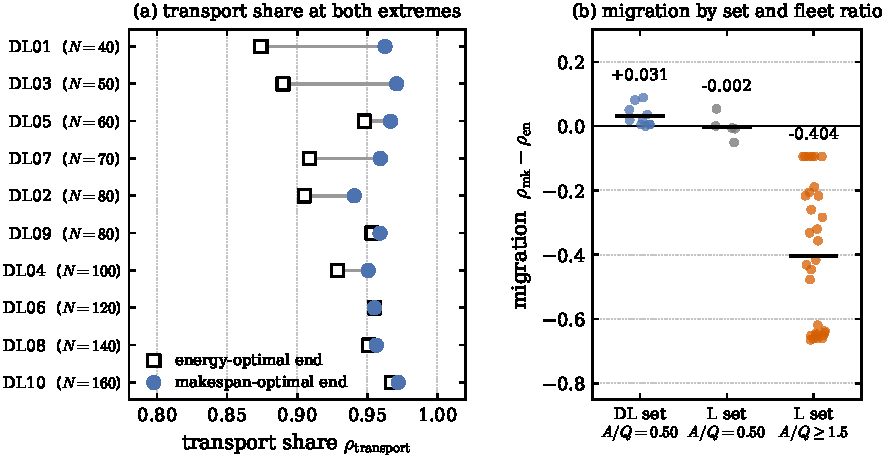
\includegraphics[width=0.80\textwidth]{figs/fig_dl.pdf}
\caption[The published large dual-cycling set]{The published large dual-cycling set, over five seeds per instance. (a) Transport share
at the two ends of every DL front, ordered by instance size. Both ends lie above $0.87$, and the
separation between them is the migration. (b) Migration for the DL set at its native
$A/Q = 0.50$, for the small instances at the same ratio, and for the small instances at
$A/Q \geq 1.5$, with group means marked. The first two groups are comparable in magnitude and
the third is not. The decomposition closes on all $50$ DL replicates.}
\label{fig:dl}
\end{figure}

\section{Bottleneck migration across the fleet-to-crane ratio}
\label{sec:migration}

Table~\ref{tab:migration} reports the sweep and Figure~\ref{fig:migration} plots it, one panel
per instance. Migration differs significantly from zero in 45 of the 54 instance--fleet cells
after Holm correction, and the pattern is consistent across instances: negligible at low ratios,
rising sharply near unity, and saturating thereafter.

% ---- BEGIN generated: tables/migration.tex (scripts/make_thesis_tables.py) ----
% Generated by scripts/make_thesis_tables.py -- do not edit by hand.
\begin{table}[tb]
\centering
\small
\caption[Bottleneck migration across the fleet-to-crane ratio]{Bottleneck migration across the fleet size, for the six swept instances. Migration is the signed shift of the duration-weighted transport share, $\rho_{\mathrm{mk}} - \rho_{\mathrm{en}}$, on the exact critical path, each cell the mean over ten seeds. Beneath each cell the model's own migration is given, and beneath that the ratio $A/Q$ followed by the mean absolute difference $|\\Delta\\rho|$ between the two. The ratio differs between instances because the crane count does. Parenthesised cells are those not significant at $\alpha = 0.05$ under a one-sample Wilcoxon signed-rank test against zero, Holm-corrected within each instance's nine fleet sizes. Migration is negligible left of $A/Q \approx 1$ and saturates to its right.}
\label{tab:migration}
\footnotesize
\setlength{\tabcolsep}{4pt}
\begin{tabular}{lrrrrrrrrr}
\toprule
Instance & \multicolumn{9}{c}{fleet size $A$, with $A/Q$ beneath} \\
\cmidrule(l){2-10}
 & 1 & 2 & 3 & 4 & 5 & 6 & 7 & 8 & 9 \\
\midrule
L01 & $-0.051$ & $+0.108$ & $-0.432$ & $-0.094$ & $-0.094$ & $-0.094$ & $-0.094$ & $-0.094$ & $-0.094$ \\
\hspace{1.2em}\tiny model & \tiny $-0.051$ & \tiny $+0.100$ & \tiny $-0.432$ & \tiny $-0.094$ & \tiny $-0.095$ & \tiny $-0.095$ & \tiny $-0.095$ & \tiny $-0.095$ & \tiny $-0.096$ \\
 & \tiny 0.50, 0.001 & \tiny 1.00, 0.012 & \tiny 1.50, 0.001 & \tiny 2.00, 0.001 & \tiny 2.50, 0.001 & \tiny 3.00, 0.001 & \tiny 3.50, 0.001 & \tiny 4.00, 0.001 & \tiny 4.50, 0.001 \\[1.5pt]
L07 & ($+0.000$) & $-0.088$ & $-0.660$ & $-0.648$ & $-0.654$ & $-0.651$ & $-0.638$ & $-0.643$ & $-0.619$ \\
\hspace{1.2em}\tiny model & \tiny $-0.000$ & \tiny $-0.104$ & \tiny $-0.606$ & \tiny $-0.648$ & \tiny $-0.611$ & \tiny $-0.652$ & \tiny $-0.574$ & \tiny $-0.561$ & \tiny $-0.615$ \\
 & \tiny 0.50, 0.001 & \tiny 1.00, 0.017 & \tiny 1.50, 0.055 & \tiny 2.00, 0.001 & \tiny 2.50, 0.044 & \tiny 3.00, 0.002 & \tiny 3.50, 0.065 & \tiny 4.00, 0.083 & \tiny 4.50, 0.006 \\[1.5pt]
L15 & $-0.008$ & ($+0.056$) & $-0.321$ & $-0.357$ & $-0.260$ & $-0.217$ & $-0.217$ & $-0.189$ & $-0.206$ \\
\hspace{1.2em}\tiny model & \tiny $-0.008$ & \tiny $+0.044$ & \tiny $-0.254$ & \tiny $-0.353$ & \tiny $-0.239$ & \tiny $-0.213$ & \tiny $-0.155$ & \tiny $-0.186$ & \tiny $-0.177$ \\
 & \tiny 0.50, 0.000 & \tiny 1.00, 0.013 & \tiny 1.50, 0.156 & \tiny 2.00, 0.004 & \tiny 2.50, 0.022 & \tiny 3.00, 0.004 & \tiny 3.50, 0.062 & \tiny 4.00, 0.003 & \tiny 4.50, 0.061 \\[1.5pt]
L21 & $-0.235$ & $-0.247$ & $-0.658$ & $-0.664$ & $-0.662$ & $-0.661$ & $-0.651$ & $-0.665$ & $-0.646$ \\
\hspace{1.2em}\tiny model & \tiny $-0.203$ & \tiny $-0.239$ & \tiny $-0.470$ & \tiny $-0.660$ & \tiny $-0.655$ & \tiny $-0.656$ & \tiny $-0.647$ & \tiny $-0.662$ & \tiny $-0.646$ \\
 & \tiny 0.33, 0.032 & \tiny 0.67, 0.028 & \tiny 1.00, 0.187 & \tiny 1.33, 0.004 & \tiny 1.67, 0.007 & \tiny 2.00, 0.005 & \tiny 2.33, 0.005 & \tiny 2.67, 0.003 & \tiny 3.00, 0.007 \\[1.5pt]
L28 & $-0.002$ & ($+0.054$) & $-0.063$ & ($-0.042$) & $-0.160$ & $-0.332$ & $-0.417$ & $-0.478$ & $-0.446$ \\
\hspace{1.2em}\tiny model & \tiny $-0.002$ & \tiny $+0.056$ & \tiny $-0.050$ & \tiny $-0.042$ & \tiny $-0.140$ & \tiny $-0.327$ & \tiny $-0.413$ & \tiny $-0.448$ & \tiny $-0.444$ \\
 & \tiny 0.25, 0.001 & \tiny 0.50, 0.003 & \tiny 0.75, 0.036 & \tiny 1.00, 0.001 & \tiny 1.25, 0.093 & \tiny 1.50, 0.042 & \tiny 1.75, 0.009 & \tiny 2.00, 0.032 & \tiny 2.25, 0.015 \\[1.5pt]
L35 & $-0.012$ & ($+0.007$) & ($-0.006$) & ($+0.027$) & ($-0.021$) & $-0.076$ & ($-0.109$) & $-0.257$ & $-0.284$ \\
\hspace{1.2em}\tiny model & \tiny $-0.012$ & \tiny $+0.000$ & \tiny $-0.006$ & \tiny $+0.024$ & \tiny $-0.031$ & \tiny $-0.088$ & \tiny $-0.078$ & \tiny $-0.073$ & \tiny $-0.261$ \\
 & \tiny 0.17, 0.000 & \tiny 0.33, 0.009 & \tiny 0.50, 0.001 & \tiny 0.67, 0.007 & \tiny 0.83, 0.019 & \tiny 1.00, 0.016 & \tiny 1.17, 0.031 & \tiny 1.33, 0.184 & \tiny 1.50, 0.025 \\[1.5pt]
\bottomrule
\end{tabular}
\end{table}
% ---- END generated: tables/migration.tex ----

\begin{figure}[tb]
\centering
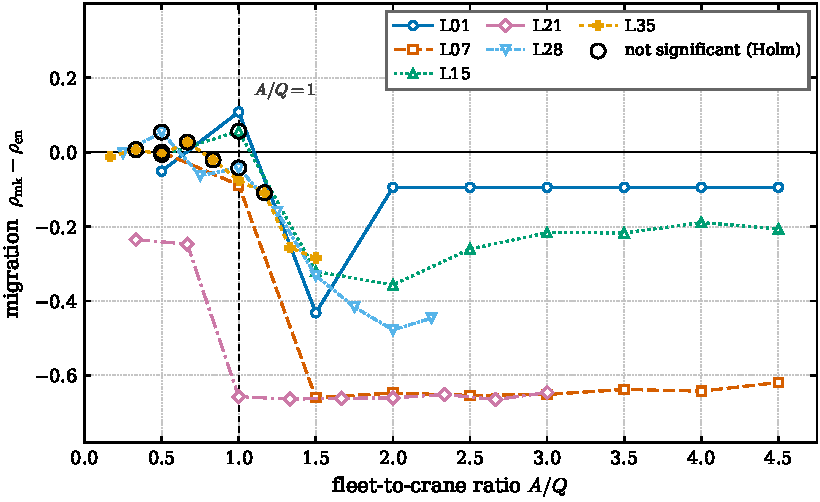
\includegraphics[width=0.78\textwidth]{figs/fig_migration.pdf}
\caption[Migration against the fleet-to-crane ratio]{Migration against the fleet-to-crane ratio for the six swept instances, each cell the
mean over ten seeds. Series are distinguished by marker and dash pattern so that they remain
separable in greyscale. Open circles mark cells that fail significance after Holm correction;
they are exactly the near-zero cells at low $A/Q$. The dashed vertical is $A/Q = 1$. The
threshold structure is the result: migration is absent below $A/Q \approx 1$, grows sharply
thereafter, and saturates. The crossing point is instance-dependent. The ratio ranges differ
by instance because nine fleet sizes are swept against a fixed crane count that differs
between them. Dispersion is omitted here and reported per cell in
Table~\ref{tab:migration}.}
\label{fig:migration}
\end{figure}

Forty-one of the 45 significant cells carry a Holm-corrected $p$ of $0.0176$, the smallest
value a ten-sample Wilcoxon test can attain, with a rank-biserial effect size of $-1.00$ in all
but seven cells; the test therefore separates the two regimes without discriminating within either. At the
lowest ratios migration is negligible. L07 at $A/Q = 0.50$ yields $+0.000$ and is one of the nine
cells failing significance, every one of which lies at $A/Q \leq 1.17$, and L15, L28 and L35 all
yield values within $0.06$ of zero below $A/Q \approx 1$. This reproduces, from independent runs, the regime of
Section~\ref{sec:degenerate} at the same ratio, which is the confirmation that section predicted.

Migration then increases sharply and saturates. L07 moves from $-0.088$ at $A/Q = 1.00$ to
$-0.660$ at $1.50$, thereafter remaining near $-0.64$ for every larger fleet. L21 attains
$-0.658$ by $A/Q = 1.00$ and holds within $0.02$ of $-0.66$ across the remaining six ratios,
peaking at $-0.665$. L28 crosses at $A/Q = 1.25$ and L35 at $1.33$, both later than L07 and L21.
The threshold is therefore instance-dependent rather than universal, which is to be expected:
whether cranes can become binding depends on handling times and layout geometry, not on the ratio
alone.

The sign identifies the direction of the transfer. Where migration is
substantial it is negative, so by Eq.~\eqref{eq:migration} the energy-optimal end is the
travel-heavy one and the bottleneck moves towards vehicle travel as energy is prioritised.
The worked case of Figure~\ref{fig:front} makes this concrete on a single replicate of that
cell: at the makespan-optimal end of L21 at $A/Q = 1.67$ the critical path is only $23.0\%$
travel and therefore predominantly crane handling, whereas at the energy-optimal end it is
$89.9\%$ travel, a migration of $-0.669$ against the cell mean of $-0.662$ in
Table~\ref{tab:migration}.

The mechanism follows from the speed selection. Minimising the makespan drives every leg to the
fastest available speed,
which compresses travel until the crane chains, whose handling times are fixed and independent
of vehicle speed, become the binding resource. Minimising energy does the reverse, selecting slow
speeds that lengthen every leg until travel dominates the path again. The cranes therefore bind at
the fast end and the vehicles at the slow end, which is why the transfer requires enough vehicles
for the cranes to be competitive in the first place, and why it vanishes below $A/Q \approx 1$.

The single instance exhibiting the opposite sign, L01 at $A/Q = 1.00$ with $+0.108$ inverted
relative to its neighbours, is the four-task instance, whose 35-point front offers too few
structurally distinct schedules for the argument to apply.

A second campaign, independent of the sweep, holds each of the 35 published small instances at
the fleet ratio its own configuration specifies and runs ten seeds of each.
Table~\ref{tab:smallset} groups its 350 replicates by ratio. The proportion whose
migration exceeds $0.1$ in magnitude rises monotonically from none at $A/Q = 0.33$ to $56\%$ at
$A/Q = 1.00$. Because the published configurations reach only $A/Q = 1.00$, this campaign
observes the sub-threshold side alone, and it corroborates the ratio dependence on the whole set
rather than on the six instances of the sweep. It also shows that the onset is gradual from
about $A/Q = 0.4$ rather than a step at unity.

% ---- BEGIN generated: tables/smallset.tex (scripts/make_thesis_tables.py) ----
% Generated by scripts/make_thesis_tables.py -- do not edit by hand.
\begin{table}[tb]
\centering
\small
\caption[Migration on the published small instances at their native ratios]{Migration on all 35 published small instances at their native fleet ratios, ten seeds each, grouped by ratio. This campaign is independent of the sweep of Table~\ref{tab:migration}, which varies the ratio on six instances; here the ratio is whatever the published configuration specifies. The proportion of replicates whose migration exceeds $0.1$ in magnitude rises monotonically with the ratio, which corroborates the dependence on a larger set of instances. The ratios reach only $1.00$, so the campaign probes the sub-threshold side alone. The decomposition closes on all 350 replicates, so none is excluded.}
\label{tab:smallset}
\footnotesize
\begin{tabular}{rrrrr}
\toprule
$A/Q$ & $n$ & mean migration & mean $|$migration$|$ & $|$migration$| > 0.1$ \\
\midrule
0.33 & 10 & $+0.007$ & 0.036 & 0\% \\
0.40 & 40 & $+0.025$ & 0.049 & 12\% \\
0.50 & 60 & $-0.010$ & 0.062 & 13\% \\
0.67 & 80 & $-0.071$ & 0.126 & 41\% \\
1.00 & 160 & $-0.110$ & 0.172 & 56\% \\
\midrule
\multicolumn{5}{l}{Overall: $n = 350$, mean $-0.065$, mean $|$migration$|$ 0.124} \\
\bottomrule
\end{tabular}
\end{table}
% ---- END generated: tables/smallset.tex ----

Several cells report a standard deviation of exactly zero across ten seeds, notably L01 throughout
and L21 at the lowest ratio. In those cells every seed recovers the same two extreme schedules,
which is unsurprising for a four-task instance and indicates saturation of the search rather than
of the measure.

\section{The three instance families}
\label{sec:families}

Every result to this point rests on the loading family: in the 35 published small instances each
of the 368 container moves is a loading task, so the unloading recurrence~\eqref{eq:unload} is
never exercised, and the dual-cycling instances of Section~\ref{sec:degenerate} are observed at a
single fleet ratio. The source supplies the remedy without further data. Loading instances are
Table~5 as printed; unloading instances are obtained from the same table by reversing the origins
and destinations, so that a container originates at the crane and is delivered to the yard
station; and a mixed instance is formed by combining one loading instance with one unloading
instance. Applying these two constructions to Table~5 yields 35 unloading and 26 mixed instances
alongside the 35 loading instances already used, on the same layout and with no value retyped.

The pairing that forms the mixed set is stated in the source: the ``comb.\ of'' column of
Table~3 names, for each of the 26 instances, the unloading and loading instance it combines. That
column is used as printed, so the family reproduces the published set rather than approximating
it. It pairs by neither adjacency nor position, D04 combining U01 with L02 and D06 combining U02
with L01, and the reconstruction is confirmed against an independent published quantity: the task
count of all 26 agrees with the Q--T column of the same table.

Each of the 96 instances was run at nine fleet sizes with ten seeds, and the transport share was
computed at every point of every resulting front rather than at the two extremes alone. The
campaign comprises 8,640 replicates and 657,899 front points; no replicate failed to complete
and the decomposition closes at every point. Table~\ref{tab:families} reports migration by ratio
for each family and Figure~\ref{fig:families} plots it.

% ---- BEGIN generated: tables/families.tex (scripts/make_thesis_tables.py) ----
% Generated by scripts/make_thesis_tables.py -- do not edit by hand.
\begin{table}[tb]
\centering
\small
\caption[Migration by fleet ratio on the three instance families]{Migration by fleet-to-crane ratio on the three instance families. Loading is Table 5 as printed; unloading is the same data with origins and destinations reversed; mixed combines one loading with one unloading instance, following the construction stated in the source. Each cell is the mean over all instances of that family and ten seeds, restricted to the ratios every family attains. The threshold is reproduced independently on all three: migration is negligible below $A/Q \approx 1$ and saturates near $-0.5$ above it. Family sizes: loading 3{,}150 replicates and 232{,}835 front points; unloading 3{,}150 replicates and 230{,}211 front points; mixed 2{,}340 replicates and 194{,}853 front points.}
\label{tab:families}
\footnotesize
\begin{tabular}{rrrr}
\toprule
$A/Q$ & loading & unloading & mixed \\
\midrule
0.25 & $-0.021$ & $-0.014$ & $-0.019$ \\
0.33 & $-0.043$ & $-0.042$ & $+0.205$ \\
0.50 & $-0.049$ & $-0.022$ & $+0.095$ \\
0.67 & $-0.060$ & $-0.023$ & $+0.075$ \\
0.75 & $-0.083$ & $-0.017$ & $-0.115$ \\
1.00 & $-0.106$ & $-0.017$ & $-0.153$ \\
1.25 & $-0.279$ & $-0.166$ & $-0.545$ \\
1.33 & $-0.359$ & $-0.207$ & $-0.197$ \\
1.50 & $-0.453$ & $-0.291$ & $-0.386$ \\
1.67 & $-0.527$ & $-0.372$ & $+0.005$ \\
1.75 & $-0.490$ & $-0.400$ & $-0.562$ \\
2.00 & $-0.497$ & $-0.469$ & $-0.410$ \\
2.25 & $-0.514$ & $-0.448$ & $-0.555$ \\
2.33 & $-0.538$ & $-0.538$ & $-0.179$ \\
2.50 & $-0.488$ & $-0.483$ & $-0.342$ \\
2.67 & $-0.550$ & $-0.530$ & $-0.179$ \\
3.00 & $-0.503$ & $-0.480$ & $-0.409$ \\
3.50 & $-0.500$ & $-0.447$ & $-0.407$ \\
4.00 & $-0.495$ & $-0.445$ & $-0.412$ \\
4.50 & $-0.473$ & $-0.445$ & $-0.409$ \\
\bottomrule
\end{tabular}
\end{table}
% ---- END generated: tables/families.tex ----

\begin{figure}[tb]
\centering
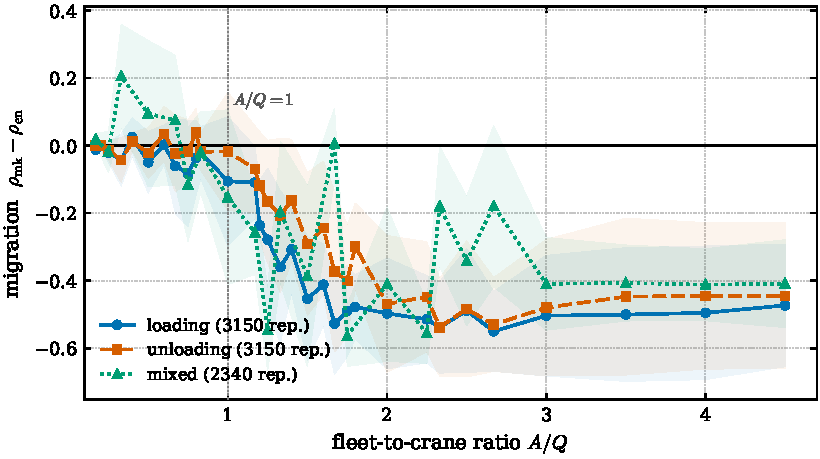
\includegraphics[width=0.78\textwidth]{figs/fig_families.pdf}
\caption[Migration on the three instance families]{Migration against the fleet-to-crane ratio on the three instance families, with the
shaded band one standard deviation across instances and seeds. The threshold is reproduced
independently on each: migration is negligible below $A/Q \approx 1$, turns sharply negative
through $1.2$ to $1.5$, and saturates near $-0.5$. The mixed family departs from the other two
below the threshold, where its migration is consistently positive rather than near zero.}
\label{fig:families}
\end{figure}

The threshold established on loading instances therefore holds on all three families. Two
differences are visible and neither follows from the mechanism of Section~\ref{sec:migration}.
Above the threshold the unloading family migrates no further than the loading family at any
ratio, the gap running from $0.09$ to $0.16$ between $A/Q = 1.25$ and $1.75$ and closing to zero
at $2.33$; the recurrences differ in where the handling term
enters the maximum, which is a candidate explanation that was not tested. Below the threshold the
mixed family carries a positive migration of up to $+0.205$ where the single-cycling families sit
near zero, so on a mixed instance with few vehicles the makespan-optimal end is the more
travel-heavy of the two. Both are reported as measured regularities and neither is claimed as
understood.

Because the share is computed at every front point rather than at the two ends, the explanation
can also be read as a profile along the front. Figure~\ref{fig:profile} shows one front from each
family.
The transition from a crane-bound to a vehicle-bound critical path occurs across the front rather
than at its ends, and it is not monotone: neighbouring points differ in which resource binds,
with the share moving by more than $0.3$ between adjacent compromises. A two-point measurement
reports the endpoints of this profile and is silent about its shape. Whether the non-monotonicity
reflects genuine structure or the search returning structurally distinct schedules at
neighbouring objective values is not resolved here.

\begin{figure}[tb]
\centering
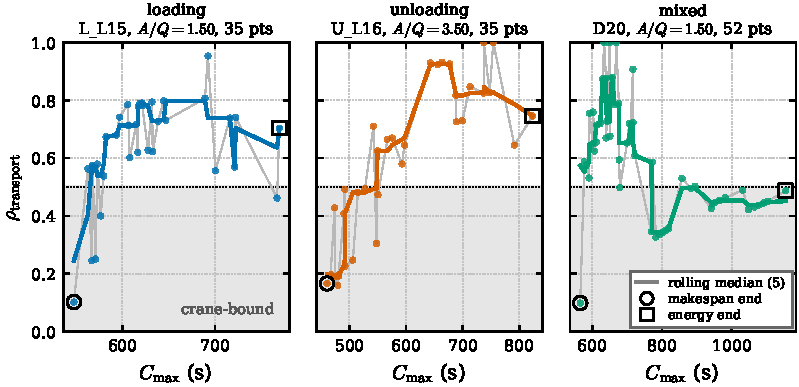
\includegraphics[width=0.78\textwidth]{figs/fig_profile.pdf}
\caption[The transport share along a front]{The transport share at every point of one front from
each family, plotted against the makespan of that point. The dotted rule at
$\rho_{\mathrm{transport}} = 0.5$ separates the crane-bound from the vehicle-bound regime. The
share rises from the makespan-optimal end to the energy-optimal end in all three, but not
monotonically.}
\label{fig:profile}
\end{figure}

\section{How the explanation changes during the search}
\label{sec:evolution}

Every result to this point explains \emph{finalised} solutions. Two questions remain open, and
they are the two roles the surrogate can take beyond post-hoc explanation. Whether the
explanation of a front is settled once the front is, or still moving while the search converges;
and whether the learned model tracks that movement, which is what any later use of it inside the
search would require.

Both are answered by snapshotting the solver's archive every ten generations. Six instances from
each of the three families are run at three fleet sizes with five seeds, giving 54 cells, 270
replicates and 2{,}970 snapshots. At every snapshot the transport share is computed twice: once
from the exact recurrence, and once from the surrogate, whose gradients are weighted by its own
predicted durations so that the two explanations are never mixed. One model is fitted per
instance and fleet size and reused across seeds, since it depends on the instance and not on the
random stream. No replicate failed.

Figure~\ref{fig:evolution} reports the first. The explanation is not settled early: above the
threshold the mean migration moves from $-0.101$ at generation zero to $-0.274$ at generation
one hundred, reaching its final value to within
$0.02$ only by generation forty; below the threshold it moves from $-0.009$ to $-0.048$ and
settles by generation thirty. An explanation read from an unconverged front therefore understates
the effect by more than half, because the early archive holds few structurally distinct schedules
and its two extremes lie close together. This is a caution rather than a defect: it establishes
that explaining \emph{finalised} solutions, which is what Section~\ref{sec:migration} does, is the
defensible use, and it gives the feedback loop of Chapter~\ref{sec:limitations} a precondition,
since guidance drawn from an early generation would act on an explanation that has not converged.

The surrogate tracks that movement closely. Over all 2{,}970 snapshots the median absolute
difference between the model's migration and the exact value is $0.0026$, and the model is
therefore reproducing the explanation while the search is still running, not only at its end. The
agreement is family-dependent and its error distribution is skewed: the median is $0.0014$ on
loading, $0.0052$ on unloading and $0.0062$ on mixed instances, but the corresponding
means are $0.022$, $0.052$ and $0.076$, and the ninetieth percentile reaches $0.347$ on the
mixed family. The model is thus accurate in the typical case and occasionally far from it,
which is the same pattern Section~\ref{sec:surrogate-eval} reports for finalised solutions and
has the same cause: where several resources are nearly balanced, a small error in a predicted
duration changes which activity binds.

A second consequence concerns the generation budget. Chapter~\ref{sec:limitations} notes that all
runs use 100 generations against the published 300; the measurements here show migration settled
well before the hundredth generation on both sides of the threshold, so the reduced budget is
sufficient for this particular measurement, whatever it costs in absolute front quality.

\begin{figure}[tb]
\centering
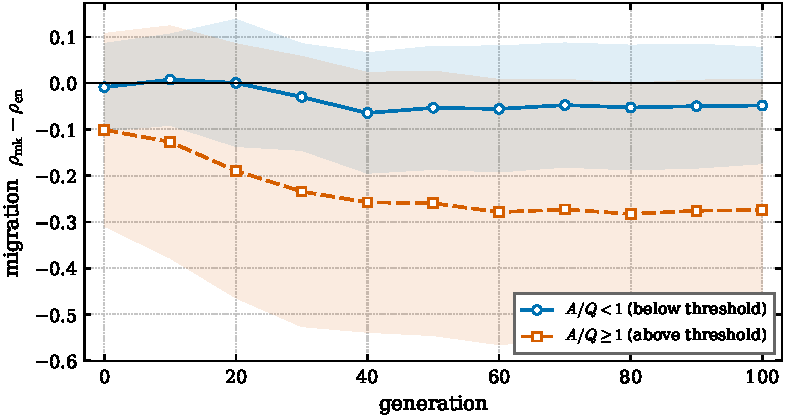
\includegraphics[width=0.78\textwidth]{figs/fig_evolution.pdf}
\caption[The explanation during the search]{Migration against generation, over 270 replicates
with the solver's archive snapshotted every ten generations, grouped by side of the
fleet-to-crane threshold with the band one standard deviation over replicates. Above the
threshold the explanation moves from $-0.101$ to $-0.274$ and reaches its final value to within
$0.02$ only by generation forty; below it there is little to settle. An explanation read from an
unconverged front is therefore biased towards zero.}
\label{fig:evolution}
\end{figure}

\section{Reproduction by the surrogate}
\label{sec:surrogate-eval}

Table~\ref{tab:calibration} reports the secondary tier: whether the learned model reproduces the
explanation that the max-plus layer supplies exactly.

% ---- BEGIN generated: tables/calibration.tex (scripts/make_thesis_tables.py) ----
% Generated by scripts/make_thesis_tables.py -- do not edit by hand.
\begin{table}[tb]
\centering
\small
\caption[Surrogate calibration and post-hoc faithfulness]{Surrogate calibration and post-hoc faithfulness over the sweep (mean over all fleet sizes and seeds per instance). These quantities belong to the secondary, over-requirements tier: they measure how well the model reproduces an explanation that the exact oracle already provides without it.}
\label{tab:calibration}
\footnotesize
\begin{tabular}{lrrrrr}
\toprule
Instance & $n$ & $R^2(C_{\max})$ & $R^2(E)$ & Leg Jaccard & $|\Delta\rho|$ \\
\midrule
L01 & 90 & 0.9991 & 1.0000 & 0.990 & 0.0022 \\
L07 & 90 & 0.9993 & 1.0000 & 0.882 & 0.0304 \\
L15 & 90 & 0.9995 & 1.0000 & 0.917 & 0.0362 \\
L21 & 90 & 0.9994 & 1.0000 & 0.885 & 0.0309 \\
L28 & 90 & 0.9994 & 1.0000 & 0.888 & 0.0258 \\
L35 & 90 & 0.9993 & 1.0000 & 0.825 & 0.0326 \\
\bottomrule
\end{tabular}
\end{table}
% ---- END generated: tables/calibration.tex ----

Calibration is high, with $R^2$ on the makespan at $0.999$ or above. The energy figure should not
be read as a success, for the architectural reason given in Section~\ref{sec:tropical}.

The meaningful quantity is the reproduction of $\rho$. The mean absolute difference between the
surrogate's migration estimate and the exact value is $0.026$ across the sweep, against migration
magnitudes reaching $0.66$, a relative error of approximately five per cent on the effect being
measured. On the cells of largest migration the discrepancy is also largest, reaching
$0.187$ on L21 at $A/Q = 1.00$, so the reproduction is weakest precisely where the
phenomenon is strongest.

That anti-correlation is the honest summary of the secondary result, and it is the reason the two
tiers are reported separately throughout. The exact explanation of
Tables~\ref{tab:traversal}--\ref{tab:migration} does not degrade when the surrogate does.

\section{Discussion}

The results support a specific and bounded claim. For this problem the reason a solution is
Pareto-optimal can be stated exactly, in seconds attributable to named physical activities, with
the attribution summing to the objective by construction. This is stronger than a feature
attribution over decision variables, and it is available because the objective possesses
$(\max,+)$ structure that the max-plus layer preserves rather than because of any technique
imported from machine learning. The architectural lesson is narrow but transferable: the encoder
was not the obstacle to faithful attribution, the pooled regression head was, and replacing that
head with the problem's own recurrence removes the obstacle without sacrificing the learned
representation.

The explanation is not static along the front. Where vehicles are sufficiently plentiful, trading
time for energy transfers the binding constraint from the cranes to the vehicles by an amount
reaching two-thirds of the critical path; where they are scarce, as in every published large
instance, it does not, there being no second candidate for the bottleneck. An operator reading a
front therefore cannot assume its members are limited by the same resource, and $A/Q$ indicates
which regime obtains. The surrogate reproduces that explanation to a mean absolute $\rho$ error of
$0.026$, with critical-leg agreement of $0.898$ on the small instances and $0.924$ on the published
large ones, and it does so least accurately where the effect is largest, since Pareto-optimal
schedules are those in which resources are nearly balanced. The exact recurrence remains the
yardstick, but it can only be applied to a schedule that has already been evaluated; the model
predicts the durations and can therefore explain a candidate before that evaluation exists, which
is the setting the feedback loop of Chapter~\ref{sec:limitations} would require.

% ======================================================================================
\chapter{Limitations and Future Work}
\label{sec:limitations}

\paragraph{Ties in the argmax.} An earlier version of the attribution produced, on a small
fraction of schedules, a critical path whose durations did not sum to the makespan. The faulty
component was not the tropical layer but the reduction after it: the makespan is a maximum over
several terminal nodes, and that reduction used the framework's own maximum operator, which
divides the incoming gradient equally between tied maxima, so each activity on both paths
inherited a fractional share and the strict on-path test admitted neither. Any single maximiser
is a valid subgradient of a maximum; an average of several is not a valid selection for an
additive decomposition. The correction selects the maximal terminal by index, restoring the
convention the recurrence already follows, and was applied at every terminal reduction including
the batched form. Across 43 non-closing schedules from seven instances of all three families
every activity gradient was at most $0.5$, so the tie accounts for every case examined. Every
affected computation was repeated from its recorded seed: the decomposition now closes on all 940
replicates and at all 657{,}899 front points, against nine replicates and $1.30\%$ of points
before, with conclusions unchanged and only one of 54 cells moving at all, by $0.001$. Why the
pre-correction failure rate differed by family, at $0.16\%$ on loading against $2.94\%$ on
unloading, was not established.

\paragraph{Scope of the claim.} All runs use 100 generations against the published $300$, which
suffices for a measurement depending on the two front extremes but places absolute front quality
below what the method attains, so no claim about front quality should be drawn here. The sweep
establishes that migration depends on $A/Q$ and locates the transition between $1.0$ and $1.35$
for four instances, but does not predict it from instance parameters. It is also established on
the small-instance layout alone: the large dual-cycling instances describe a twenty-crane terminal
whose distance matrix is not interchangeable, and are observed only at $A/Q = 0.50$, so extending
the threshold to them is an extrapolation across layouts rather than a measurement. Sweeping the
fleet on three large dual-cycling instances would settle it, at roughly forty core-hours. Finally, the
surrogate's agreement with the exact critical set is lowest where migration is largest, since
Pareto-optimal schedules are those in which resources are nearly balanced and small prediction
errors alter which activity binds; this bounds the secondary tier only.

\paragraph{Further work.} Two implemented components are excluded. A power-coupled regime, in
which a terminal-wide budget couples the vehicles, is the one setting in which the surrogate
would predict a quantity with no closed form, the waiting time induced by power contention, and
therefore where a learned component becomes necessary rather than merely sufficient; it is the
strongest candidate for future work but needs a separate problem statement, originating as it
does in a different literature. Its three-velocity configuration and power coefficients are
retained here, belonging to the original problem. The natural continuation is to feed the explanation back into the search, which divides into two
steps of unequal size. The smaller, comparing how the explanation changes across generations, is
carried out in Section~\ref{sec:evolution} and shows that an explanation read from an unconverged
front is biased towards zero. The larger is attribution-guided search proper, biasing mutation
towards the activities currently on the critical path, in the spirit of decision-focused learning
\citep{elmachtoub2022}. That step is deliberately not attempted here: it should follow once the
explanation is established, which is what this thesis does, and Section~\ref{sec:evolution} gives
it a precondition, since guidance drawn from an early generation would be acting on an
explanation that has not yet converged.

% ======================================================================================
\chapter{Conclusion}
\label{sec:conclusion}

This thesis set out to explain why particular solutions to a bi-objective container-terminal
scheduling problem are Pareto-optimal, rather than merely to compute them. Its one core idea
is that such a schedule can be explained exactly, in seconds attributable to named physical
activities, and that a learned model can produce the same explanation. The instances are the
published ones throughout: the loading set as printed, the unloading set reversed from it, and
the mixed set formed by the pairing the source states, each reconstruction checked
against the optima published for it before any result was drawn from it.

Because the makespan is a maximum of sums of activity durations, it is a longest path over the
$(\max,+)$ semiring, and the sensitivity of the makespan to each activity is exactly zero or one.
A conventional surrogate cannot express this: a pooled regression head produces a dense Jacobian
and therefore assigns credit to provably irrelevant activities. Replacing that head with a
differentiable max-plus dynamic programme, whose backward pass routes the subgradient through the
recorded argmax edge, restores the property, and differentiating the composition returns the
critical path itself rather than an estimate of it. From that decomposition the duration-weighted
critical share $\rho$ summarises an explanation as one number, the fraction of the makespan spent
moving rather than lifting.

The empirical result is that the bottleneck migrates, and that whether it does is governed by the
fleet-to-crane ratio. Across 540 statistically tested replicates migration is significantly
non-zero in 45 of 54 instance--fleet cells and attains a magnitude of $0.665$; below
$A/Q \approx 1$ it vanishes, both front extremes being transport-bound. A further 8{,}640
replicates reproduce the threshold on three instance families, so the result does not depend on
every container being a loading move. Where it occurs the cranes bind at the makespan-optimal end
and the vehicles at the energy-optimal end, which accounts for its absence on the ten published
large instances, each having $A/Q = 0.50$. The operational reading is that two schedules on one
front need not be limited by the same resource, and that the fleet ratio indicates whether an
operator is in the regime where this distinction matters.

The learned surrogate reproduces the same explanation to a mean absolute $\rho$ error of $0.026$,
with critical-leg agreement of $0.898$ on the small instances and $0.924$ on the largest published
ones at up to 160 tasks. That is what licenses the method beyond the cases examined here: the exact
recurrence is available for a resolved schedule, but it requires one, whereas the model predicts
the durations and can therefore explain a candidate that has not been evaluated. Every setting in
which the explanation is wanted before evaluation, or in which no closed form exists, rests on the
learned component rather than on the oracle.

% ======================================================================================
% A bibliography is set single-spaced with a small gap between entries; the one-and-a-half
% spacing of the body makes the entries sprawl and the block hard to scan. The contents entry
% is added at chapter level and under the heading the class actually prints, so that the list
% is not indented under the final chapter and does not appear under a different name.
\begingroup
\singlespacing\footnotesize
\setlength{\bibsep}{0.1em}
\cleardoublepage
\addcontentsline{toc}{chapter}{Bibliography}
\bibliographystyle{plainnat}
\bibliography{references}
\endgroup

\end{document}
